\documentclass[b5paper]{book}
\usepackage[
    b5paper,
		margin=2cm,
	]{geometry}
\setlength\parindent{0em}
\setlength{\parskip}{1em}

\usepackage{booktabs}
\usepackage{blindtext}

%-----------%
% XREF DICT %
%-----------%

\usepackage{pgfkeys}
\pgfkeyssetvalue{/xref dict/fig}{Figure}
\pgfkeyssetvalue{/xref dict/eq}{Equation}
\pgfkeyssetvalue{/xref dict/eqs}{Equations}
\pgfkeyssetvalue{/xref dict/tab}{Table}
\pgfkeyssetvalue{/xref dict/def}{Definition}
\pgfkeyssetvalue{/xref dict/note}{Note}
\pgfkeyssetvalue{/xref dict/challange}{Challange}
\pgfkeyssetvalue{/xref dict/example}{Example}

%----------%
% GRAPHICS %
%----------%

\usepackage{caption}
\usepackage{subcaption}

\usepackage{tikz}
\usepackage{tikzpagenodes}
\usetikzlibrary{positioning, calc, decorations.pathreplacing, decorations.text}

\tikzset{
	arrow/.style={thick, ->, >=stealth},
	vector/.style={very thick, ->, >=stealth},
}

\usepackage{pgfplots}
\usepgfplotslibrary{fillbetween, colormaps, colorbrewer}
\pgfplotsset{
		compat=1.16,
		every axis/.append style={
			font=\small,
		},
		graph2d/.style={
		axis x line=middle,
		axis y line=middle,
		every axis x label/.style={
			at={(ticklabel* cs:1.01)},
			anchor=west,
		},
		every axis y label/.style={
			at={(ticklabel* cs:1.01)},
			anchor=south,
		},
		axis line style={stealth-stealth, thick},
		label style={font=\large},
		xlabel=$x$,
		ylabel=$y$,
		tick label style={font=\small},
		samples=200,
		grid=both,
		grid style={line width=.1pt, draw=gray!20},
		major grid style={line width=.2pt,draw=gray!50},
		minor tick num=4,
	},
	function/.style={line width=1.5pt},
}

%-------%
% FONTS %
%-------%

\usepackage{kpfonts}

%--------%
% COLORS %
%--------%

\usepackage{xcolor}
\usepackage{colortbl}
\definecolor{xblue}{HTML}{4268BD}
\definecolor{xred}{HTML}{BD4242}
\definecolor{xgreen}{HTML}{52B256}
\definecolor{xpurple}{HTML}{7F52B2}
\definecolor{xorange}{HTML}{FF9F31}
\definecolor{xdotted}{HTML}{999999}

% Document-specific colors
\colorlet{normaltextcolor}{black}
\colorlet{figtextcolor}{xblue}

%------- %
% XHFILL %
%------- %

\usepackage{xhfill}

%---------------%
% CHAPTER TITLE %
%---------------%

% Used to set chapter title look.
% "explicit" is there so we can
% use the first parameter (#1).
\usepackage[explicit]{titlesec}
\newcommand{\chapternumsize}{\fontsize{70}{70}\selectfont}
\newcommand{\chaptertitlesize}{\fontsize{30}{30}\selectfont}

\titleformat{\chapter}{\sffamily\bfseries}{}{0pt}{
	\centering
	\begin{tikzpicture}[font=\sffamily\bfseries]
		\fill[black!10, rounded corners] (0,0) rectangle (5cm,5cm);
		\node (chapternum) at (2.5cm,4.5cm) {\fontsize{85}{85}\selectfont\thechapter};
		\node[below of=chapternum, yshift=-2cm] {
\includegraphics[scale=1.5]{figures/chapters/tapir_rainbow.pdf}};
		\node[align=center, below of=chapternum, yshift=-5cm] {\fontsize{30}{30}\selectfont\uppercase{#1}};
		\node[align=center, above of=chapternum, yshift=5mm] {\huge CHAPTER};
	\end{tikzpicture}
}

\titleformat{\section}{\sffamily\Large\bfseries}{\huge{\thesection}}{1em}{\uppercase{#1}}

\titleformat{\subsection}{\sffamily\large\bfseries}{}{0em}{\uppercase{#1}}

%------------%
% REFERENCES %
%------------%
\usepackage{chngcntr}
\counterwithin{table}{chapter}
\counterwithin{figure}{chapter}
\renewcommand{\eqref}[1]{
	Equation \ref{eq:#1}
}
\newcommand{\tabref}[1]{
	\textbf{\textcolor{xblue}{Table} \ref{tab:#1}}
}
\newcommand{\figref}[1]{
	\textbf{\textcolor{xblue}{Figure} \ref{fig:#1}}
}
\newcommand{\noteref}[1]{
	\textbf{\textcolor{xred}{Note} \ref{note:#1}}
}
\newcommand{\exampleref}[1]{
	\textbf{\textcolor{xblue}{Example} \ref{example:#1}}
}

%---------%
% HEADERS %
%---------%

\usepackage{fancyhdr}
\pagestyle{fancy}
\fancyhf{}% Clear header/footer
\renewcommand{\chaptermark}[1]{\markboth{\chaptername\ \thechapter:\ #1}{}}
\fancyhead[RO,LE]{\leftmark}% Chapter details in book
\fancyfoot[RO,LE]{\thepage}
\makeatother

%-------%
% BOXES %
%-------%

\usepackage{fontawesome}
\usepackage[most]{tcolorbox}
\tcbset{
	common/.style={
		lower separated=false,
		coltitle=white,
		colback=gray!5,
		boxrule=0.5pt,
		fonttitle=\bfseries,
		enhanced,
		breakable,
		top=8pt,
		before skip=8pt,
		attach boxed title to top left={
			yshift=-0.25cm,
		xshift=0.38cm},
		boxed title style={
			boxrule=0pt,
			colframe=white,
			arc=0pt,
		outer arc=0pt},
	separator sign={~~},},
	defstyle/.style={
		common,
		colframe=xpurple,
		colback=xpurple!5,
		colbacktitle=xpurple,
		overlay unbroken and last={
			\node[anchor=south east, outer sep=0pt] at (\linewidth-width, 0) {
	\textcolor{xpurple}{$\pi$}};}},
	exmplstyle/.style={
		common,
		colframe=xblue,
		colback=xblue!5,
		colbacktitle=xblue,
		overlay unbroken and last={
			\node[anchor=south east, outer sep=0pt, font=\large\bfseries] at (\linewidth-width, 1) {
	\textcolor{xblue}{\faArrowCircleDown}};}},
	notestyle/.style={
		common,
		colframe=xred,
		colback=xred!5,
		colbacktitle=xred,
		overlay unbroken and last={
			\node[anchor=south east, outer sep=0pt, font=\large\bfseries] at (\linewidth-width, 1) {
	\textcolor{xred}{!}};}},
	chllngstyle/.style={
		common,
		colframe=xgreen,
		colback=xgreen!5,
		colbacktitle=xgreen,
		overlay unbroken and last={
			\node[anchor=south east, outer sep=0pt, font=\large\bfseries] at (\linewidth-width, 0) {
	\textcolor{xgreen}{?}};}},
	thmstyle/.style={
		common,
		colframe=second,
		colback=second!5,
		colbacktitle=second,
		overlay unbroken and last={
			\node[anchor=south east, outer sep=0pt] at (\linewidth-width,0) {
	\textcolor{second}{$\heartsuit$}};}},
	theoremstyle/.style={
		common,
		colframe=xpurple,
		colback=xpurple!5,
		colbacktitle=xpurple,
		overlay unbroken and last={
			\node[anchor=south east, outer sep=0pt, font=\large\bfseries] at (\linewidth-width, 1) {
	\textcolor{xpurple}{$\multimapdotbothA$}};}},
}
\newtcbtheorem[auto counter, number within=chapter]{definition}{Definition}{defstyle}{def}
\newtcbtheorem[auto counter, number within=chapter]{example}{Example}{exmplstyle}{example}
\newtcbtheorem[auto counter, number within=chapter]{note}{Note}{notestyle}{note}
\newtcbtheorem[auto counter, number within=chapter]{challange}{Challange}{chllngstyle}{challange}
\newtcbtheorem[auto counter, number within=chapter]{theorem}{Theorem}{theoremstyle}{theorem}

%---------%
% FIGURES %
%---------%

\usepackage{float}
\usepackage{caption}
\usepackage[colorlinks=true, linkcolor=xblue]{hyperref}

% Caption label
\DeclareCaptionLabelSeparator{doublespace}{\ \ }
\captionsetup{labelfont={color=xblue,bf}, figurename=Figure, labelsep=doublespace}

% Refs format
\newcommand{\xref}[2][fig]{
	\color{figtextcolor}\textbf{\pgfkeysvalueof{/xref dict/#1}}~\ref{#1:#2} \color{normaltextcolor}
}

%-------------------%
% HIGHLIGHTED WORDS %
%-------------------%

\usepackage{imakeidx}
\usepackage{marginnote}
\makeindex
\renewcommand\emph[1]{\color{xpurple}{\textbf{#1}}\color{normaltextcolor}\index{#1}}%\marginnote[#1]{}

%-------%
% MATHS %
%-------%

\usepackage{amsmath, bm}
\numberwithin{equation}{chapter}
\usepackage{siunitx}
\newcommand{\Rs}[1]{\mathbb{R}^{#1}}
%\newcommand{\true}{\colorbox{xblue!25}{true}}
%\newcommand{\false}{\colorbox{xred!25}{false}}
\newcommand{\true}{\textcolor{xblue}{\textbf{true}}}
\newcommand{\false}{\textcolor{xred}{\textbf{false}}}
\newcommand{\AND}{\textbf{AND}}
\newcommand{\OR}{\textbf{OR}}
\newcommand{\opand}{\wedge}
\newcommand{\opor}{\vee}
\newcommand{\falseprop}[1]{
	\begingroup
	\color{xred}
	\underset{\false}{#1}
	\endgroup
}
\newcommand{\trueprop}[1]{
	\begingroup
	\color{xblue}
	\underset{\true}{#1}
	\endgroup
}
\newcommand{\defeq}{:=}
\newcommand{\eqdef}{=:}
\newcommand{\conj}[1]{\overline{#1}}

%-------------%
% OTHER STUFF %
%-------------%

\usepackage[version=4]{mhchem} % for chemistry
\newcommand{\shrug}[1][]{% shrug emoji
	\begin{tikzpicture}[baseline,x=0.8\ht\strutbox,y=0.8\ht\strutbox,line width=0.125ex,#1]
		\def\arm{(-2.5,0.95) to (-2,0.95) (-1.9,1) to (-1.5,0) (-1.35,0) to (-0.8,0)};
		\draw \arm;
		\draw[xscale=-1] \arm;
		\def\headpart{(0.6,0) arc[start angle=-40, end angle=40,x radius=0.6,y radius=0.8]};
		\draw \headpart;
		\draw[xscale=-1] \headpart;
		\def\eye{(-0.075,0.15) .. controls (0.02,0) .. (0.075,-0.15)};
		\draw[shift={(-0.3,0.8)}] \eye;
		\draw[shift={(0,0.85)}] \eye;
% draw mouth
		\draw (-0.1,0.2) to [out=15,in=-100] (0.4,0.95);
\end{tikzpicture}
}

%----------%
% DOCUMENT %
%----------%

\begin{document}

% Chapters
\setcounter{chapter}{-1}

% Introduction
\pgfkeys{
	/pgfplots/Interval/.style={
	axis x line=middle,
	axis y line=none,
	every axis x label/.style={
		at={(ticklabel* cs:1.05)},
		anchor=west,
	},
	axis line style={stealth-stealth, thick},
	label style={font=\large},
	tick label style={font=\small},
	samples=200,
	xmin=-5, xmax=5,
	ymin=0, ymax=5,
	domain=-5:5,
	y=0.5cm,
	restrict y to domain=0:4,
	axis lines=left,
	enlarge x limits=upper,
	scatter/classes={o={mark=*,fill=white}},
	scatter,
	scatter src=explicit symbolic,
	every axis plot post/.style={mark=*,thick},
}}

\chapter{Introduction}\label{chapter:intro}
In this chapter we introduce key concepts that will be used in later chapters. For this reason, unlike other chapters it contains many statements, sometimes given without thorough explainations or reasoning. While all of these statements are grounded in deep ideas and can be formulated in a rigorous manner, it is adviced to first get an intuitive understanding of the ideas before diving into their more formal construction.

\vspace{2em}
\begin{note}{In case you are already familiar with the topics}{}
	It is recommended for readers who are familiar with the topics to at least gloss over this chapter and make sure they know and understand all the concept presented here.
\end{note}

%\input{chapters/intro/math_symbols_sets.tex}
%\section{Relations and Functions}
\subsection{Basics}
The Cartesian product of two sets can be viewed as describing all possible connections between the elements of the first set to the elements of the second set, and thus any subset of a Cartesian product forms a specific \emph{relation} between the sets.

\begin{example}{Relations as subsets of Cartesian products}{relation}
	Given the following two sets:
	\[
		A=\{1,2,3,4\},\ B=\{\alpha,\beta,\gamma\},
	\]
	then
	\begin{align*}
		A\times B = \left\{ (1,\alpha),\ (1,\beta),\ (1,\gamma), \right.\\
												(2,\alpha),\ (2,\beta),\ (2,\gamma),\\
												(3,\alpha),\ (3,\beta),\ (3,\gamma),\\
							  \left.	(4,\alpha),\ (4,\beta),\ (4,\gamma) \right\}.
	\end{align*}

	We can choose the following pairs to form a subset of $A\times B$:
	\[
		R = \left\{ (1,\beta),\ (2,\alpha),\ (3,\alpha),\ (3,\beta), (4,\gamma)  \right\}.
	\]
	$R$ is thus a relation between $A$ and $B$. We can graphically illustrate $R$ as follows:
	\begin{figure}[H]
		\centering
		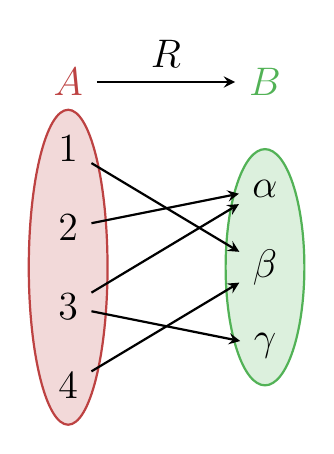
\begin{tikzpicture}
			\Large
			
			\draw[thick, xred, fill=xred!20] (0,0) ellipse (0.5cm and 2cm) node[above, yshift=2cm] (Albl) {$A$};
			\node (1) at (0,1.5cm) {$1$};
			\node (2) at (0,0.5cm) {$2$};
			\node (3) at (0,-0.5cm) {$3$};
			\node (4) at (0,-1.5cm) {$4$};
			
			\draw[thick, xgreen, fill=xgreen!20] (2.5cm,0) ellipse (0.5cm and 1.5cm) node[above, yshift=2cm] (Blbl) {$B$};
			\node (alpha) at (2.5cm,1cm) {$\alpha$};
			\node (beta) at (2.5cm,0cm) {$\beta$};
			\node (gamma) at (2.5cm,-1cm) {$\gamma$};

			\draw[arrow] (1) -- (beta);
			\draw[arrow] (2) -- (alpha);
			\draw[arrow] (3) -- (alpha);
			\draw[arrow] (3) -- (gamma);
			\draw[arrow] (4) -- (beta);

			\draw[arrow] (Albl) -- (Blbl) node[midway, above] {$R$};
		\end{tikzpicture}
	\end{figure}
\end{example}

Relations can be inversed by reversing the order of each of its pairs.

\begin{example}{Inverse relation}{inv_relation}
	The inverse relation to the relation in \autoref{example:relation} is
	\[
		R^{-1} = \left\{ (\beta,1),\ (\alpha,2),\ (\alpha,3),\ (\beta,3), (\gamma,4)  \right\}.
	\]
	Graphically:
	\begin{figure}[H]
		\centering
		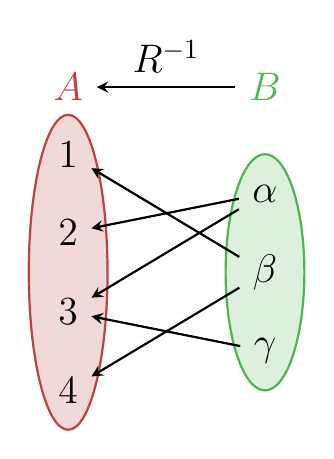
\begin{tikzpicture}
			\Large
			
			\draw[thick, xred, fill=xred!20] (0,0) ellipse (0.5cm and 2cm) node[above, yshift=2cm] (Albl) {$A$};
			\node (1) at (0,1.5cm) {$1$};
			\node (2) at (0,0.5cm) {$2$};
			\node (3) at (0,-0.5cm) {$3$};
			\node (4) at (0,-1.5cm) {$4$};
			
			\draw[thick, xgreen, fill=xgreen!20] (2.5cm,0) ellipse (0.5cm and 1.5cm) node[above, yshift=2cm] (Blbl) {$B$};
			\node (alpha) at (2.5cm,1cm) {$\alpha$};
			\node (beta) at (2.5cm,0cm) {$\beta$};
			\node (gamma) at (2.5cm,-1cm) {$\gamma$};

			\draw[arrow] (beta) -- (1);
			\draw[arrow] (alpha) -- (2);
			\draw[arrow] (alpha) -- (3);
			\draw[arrow] (gamma) -- (3);
			\draw[arrow] (beta) -- (4);

			\draw[arrow] (Blbl) -- (Albl) node[midway, above] {$R^{-1}$};
		\end{tikzpicture}
	\end{figure}
\end{example}

A \emph{function} $f$ from a set $A$ to a set $B$ is a relation for which any element in $A$ is connected to a single element in $B$.

\begin{example}{Functions}{functions}
	The following are two functions from the set $A$ to the set $B$ defined in \autoref{example:relation}:
	\begin{figure}[H]
		\centering
		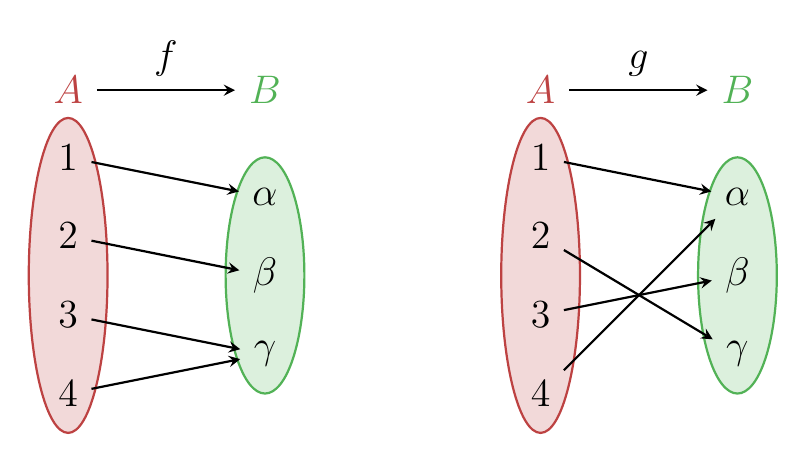
\begin{tikzpicture}
			\Large
			% f
			\draw[thick, xred, fill=xred!20] (0,0) ellipse (0.5 and 2) node[above, yshift=2cm] (Albl) {$A$};
			\node (1f) at (0,1.5) {$1$};
			\node (2f) at (0,0.5) {$2$};
			\node (3f) at (0,-0.5) {$3$};
			\node (4f) at (0,-1.5) {$4$};
			
			\draw[thick, xgreen, fill=xgreen!20] (2.5,0) ellipse (0.5 and 1.5) node[above, yshift=2cm] (Blbl) {$B$};
			\node (alpha_f) at (2.5,1) {$\alpha$};
			\node (beta_f) at (2.5,0) {$\beta$};
			\node (gamma_f) at (2.5,-1) {$\gamma$};

			\draw[arrow] (1f) -- (alpha_f);
			\draw[arrow] (2f) -- (beta_f);
			\draw[arrow] (3f) -- (gamma_f);
			\draw[arrow] (4f) -- (gamma_f);

			\draw[arrow] (Albl) -- (Blbl) node[midway, above] {$f$};
			
			% g
			\draw[thick, xred, fill=xred!20] (6,0) ellipse (0.5 and 2) node[above, yshift=2cm] (Albl) {$A$};
			\node (1g) at (6,1.5)  {$1$};
			\node (2g) at (6,0.5)  {$2$};
			\node (3g) at (6,-0.5) {$3$};
			\node (4g) at (6,-1.5) {$4$};
			
			\draw[thick, xgreen, fill=xgreen!20] (8.5,0) ellipse (0.5 and 1.5) node[above, yshift=2cm] (Blbl) {$B$};
			\node (alpha_g) at (8.5,1) {$\alpha$};
			\node (beta_g) at  (8.5,0) {$\beta$};
			\node (gamma_g) at (8.5,-1) {$\gamma$};

			\draw[arrow] (1g) -- (alpha_g);
			\draw[arrow] (2g) -- (gamma_g);
			\draw[arrow] (3g) -- (beta_g);
			\draw[arrow] (4g) -- (alpha_g);

			\draw[arrow] (Albl) -- (Blbl) node[midway, above] {$g$};
		\end{tikzpicture}
	\end{figure}
		
	The pairs making up $f$ are $(1,\alpha),\ (2,\beta),\ (3,\gamma)$ and $(4,\gamma)$, and the pairs making up $g$ are $(1,\alpha),\ (2,\gamma),\ (3,\beta)$ and $(4,\alpha)$.
\end{example}

\begin{note}{Relations which are not functions}{}
	Note that the relation in \autoref{example:relation} is \textbf{not} a function, since the element $3\in A$ is connected to more than one element in $B$, namely $\alpha$ and $\gamma$.
\end{note}

Different names are used in some branches of mathematics to describe functions, such as \emph{maps} and \emph{transformations}. Barring context, they all mean the same thing.

A common way to denote that a function $f$ is connecting elements in $A$ to elements in $B$ is
\begin{equation}
	f: A\to B.
	\label{eq:function_basics}
\end{equation}
$A$ is called the \emph{domain} of $f$, and $B$ its \emph{image}. In this book and many other sources, the following notation is used: $f(x)=y$, which means that when we apply the function $f$ to an element $x\in A$, the result is the element it is connected to, i.e. $y\in B$. We write this as $x\mapsto y$ (the special symbol $\mapsto$ is called a \emph{mapping notation}).

\begin{example}{Value $\mapsto$ value notation for functions}{}
	For the functions $f,g$ as defined in \autoref{example:functions}:
	\begin{align*}
		&f(1)=\alpha,\ f(2)=\beta,\ f(3)=f(4)=\gamma.\\
		&g(1)=g(4)=\alpha,\ g(2)=\gamma,\ g(3)=\beta.
	\end{align*}
\end{example}

\subsection{Injective, surjective and bijective functions}
A function is \emph{injective} if each of the elements in its \textbf{image} is connected to by at most a single element in its \textbf{domain}. An injective function is also known as an \emph{injection}.

\begin{example}{Injective function}{injective}
	\centering
	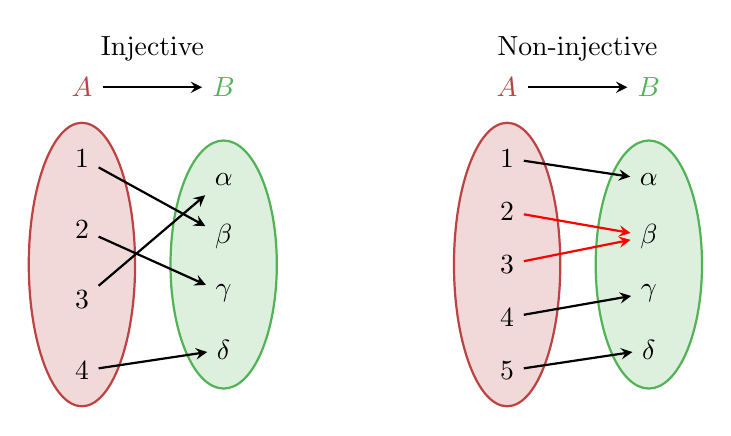
\begin{tikzpicture}[scale=0.9]
% Injective function
		\fill[xred!20, draw=xred, thick] (0,0) circle (0.75cm and 2cm) node[above, yshift=2cm, text=xred] (A) {$A$};
		\node (A1) at (0,1.5) {$1$};
		\node (A2) at (0,0.5) {$2$};
		\node (A3) at (0,-0.5) {$3$};
		\node (A4) at (0,-1.5) {$4$};

		\fill[xgreen!20, draw=xgreen, thick] (2,0) circle (0.75cm and 1.75cm) node[above, yshift=2cm, text=xgreen] (B) {$B$};
		\node (B1) at (2,1.2) {$\alpha$};
		\node (B2) at (2,0.4) {$\beta$};
		\node (B3) at (2,-0.4) {$\gamma$};
		\node (B4) at (2,-1.2) {$\delta$};

		\draw[arrow] (A1) -- (B2);
		\draw[arrow] (A2) -- (B3);
		\draw[arrow] (A3) -- (B1);
		\draw[arrow] (A4) -- (B4);

		\draw[arrow] (A) to node[midway, above, yshift=2mm] {Injective} (B);

% Non injective function
		\fill[xred!20, draw=xred, thick] (6,0) circle (0.75cm and 2cm) node[above, yshift=2cm, text=xred] (A) {$A$};
		\node (A1b) at (6,1.5) {$1$};
		\node (A2b) at (6,0.75) {$2$};
		\node (A3b) at (6,0) {$3$};
		\node (A4b) at (6,-0.75) {$4$};
		\node (A5b) at (6,-1.5) {$5$};

		\fill[xgreen!20, draw=xgreen, thick] (8,0) circle (0.75cm and 1.75cm) node[above, yshift=2cm, text=xgreen] (B) {$B$};
		\node (B1b) at (8,1.2) {$\alpha$};
		\node (B2b) at (8,0.4) {$\beta$};
		\node (B3b) at (8,-0.4) {$\gamma$};
		\node (B4b) at (8,-1.2) {$\delta$};

		\draw[arrow] (A1b) -- (B1b);
		\draw[arrow, red] (A2b) -- (B2b);
		\draw[arrow, red] (A3b) -- (B2b);
		\draw[arrow] (A4b) -- (B3b);
		\draw[arrow] (A5b) -- (B4b);

		\draw[arrow] (A) to node[midway, above, yshift=2mm] {Non-injective} (B);
	\end{tikzpicture}

	\flushleft
	The function on the right in non-injective because the element $\beta\in B$ is connected to by two elements in $A$ ($2$ and $3$, red arrows).
\end{example}

A function is \emph{surjective} if every element in its image is connected to by at least a single element in its domain (see \autoref{example:surjective}). As with injective functions, a surjective function is also known as a \emph{surjection}. A non surjective function can be made into surjective function by excluding from its image any element that is not connected to by any element from its domain (see \autoref{example:surjectification}).

A function $f:A\to B$ that is both surjective and bijective is called a \emph{bijective function} (also a \emph{bijection}). All elements in the image of a bijection are connected to by exactly a single element in its domain. This means that the direction of the connections can be flipped, yielding the \emph{inverse} of the original function (denoted $f^{-1}$).

The reason only bijective functions have inverses is as follows: Given a function $f:A\to B$,
\begin{itemize}
	\item if $f$ is non-injective, then there is at least one element $y_{1}\in B$ which is connected to by at least two elements from $A$. We can name these elements $x_{1}$ and $x_{2}$. When inverted, $f^{-1}:B\to A$ has an element $y_{1}\in B$ (note that for $f^{-1}$, $B$ is its domain), which is connected to two or more elements in $A$, the image of $f^{-1}$. These are of course $x_{1},x_{2}$. This fact disqualifies $f^{-1}$ from being a function.
	\item If $f$ is non-surgetive, then there exists at least one element $y_{2}\in B$ that is not connected to by any element from $A$. When inverted, $y_{2}$ in the domain $B$ of $f^{-1}$ is not connected to any element in its image $A$. This fact disqualifies $f^{-1}$ from being a function.
\end{itemize}

\blindtext

\begin{example}{Surjective function}{surjective}
	\centering
	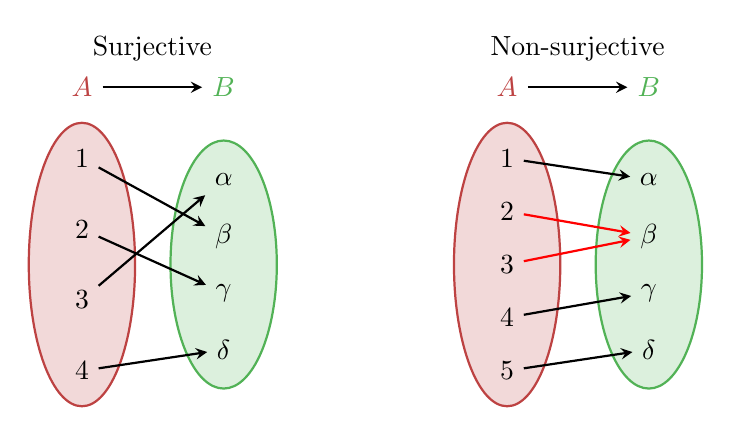
\begin{tikzpicture}[scale=0.9]
		% Surjection
		\fill[xred!20, draw=xred, thick] (0,0) circle (0.75cm and 2cm) node[above, yshift=2cm, text=xred] (A) {$A$};
		\node (A1) at (0,1.5) {$1$};
		\node (A2) at (0,0.5) {$2$};
		\node (A3) at (0,-0.5) {$3$};
		\node (A4) at (0,-1.5) {$4$};

		\fill[xgreen!20, draw=xgreen, thick] (2,0) circle (0.75cm and 1.75cm) node[above, yshift=2cm, text=xgreen] (B) {$B$};
		\node (B1) at (2,1.2) {$\alpha$};
		\node (B2) at (2,0.4) {$\beta$};
		\node (B3) at (2,-0.4) {$\gamma$};
		\node (B4) at (2,-1.2) {$\delta$};

		\draw[arrow] (A1) -- (B2);
		\draw[arrow] (A2) -- (B3);
		\draw[arrow] (A3) -- (B1);
		\draw[arrow] (A4) -- (B4);

		\draw[arrow] (A) to node[midway, above, yshift=2mm] {Surjective} (B);

		% Non surjection
		\fill[xred!20, draw=xred, thick] (6,0) circle (0.75cm and 2cm) node[above, yshift=2cm, text=xred] (A) {$A$};
		\node (A1b) at (6,1.5) {$1$};
		\node (A2b) at (6,0.75) {$2$};
		\node (A3b) at (6,0) {$3$};
		\node (A4b) at (6,-0.75) {$4$};
		\node (A5b) at (6,-1.5) {$5$};

		\fill[xgreen!20, draw=xgreen, thick] (8,0) circle (0.75cm and 1.75cm) node[above, yshift=2cm, text=xgreen] (B) {$B$};
		\node (B1b) at (8,1.2) {$\alpha$};
		\node (B2b) at (8,0.4) {$\beta$};
		\node (B3b) at (8,-0.4) {$\gamma$};
		\node (B4b) at (8,-1.2) {$\delta$};

		\draw[arrow] (A1b) -- (B1b);
		\draw[arrow, red] (A2b) -- (B2b);
		\draw[arrow, red] (A3b) -- (B2b);
		\draw[arrow] (A4b) -- (B3b);
		\draw[arrow] (A5b) -- (B4b);

		\draw[arrow] (A) to node[midway, above, yshift=2mm] {Non-surjective} (B);
	\end{tikzpicture}
\end{example}

\begin{example}{Making a non-surjective function into a surjection}{surjectification}
	Given the two sets $A=\{1,2,3,4\}$ and $B=\{\alpha,\beta,\gamma,\delta\}$, the following non-surjective function $f:A\to B$ is defined:
	\[
		f = \left\{ (1,\alpha),\ (2,\beta),\ (3,\gamma),\ (4,\gamma) \right\}.
	\]

	By removing $\delta$ from $B$, the function $f$ becomes surjective (though it remains non-injective).
\end{example}

\begin{example}{Cross examples}{}
	\centering
	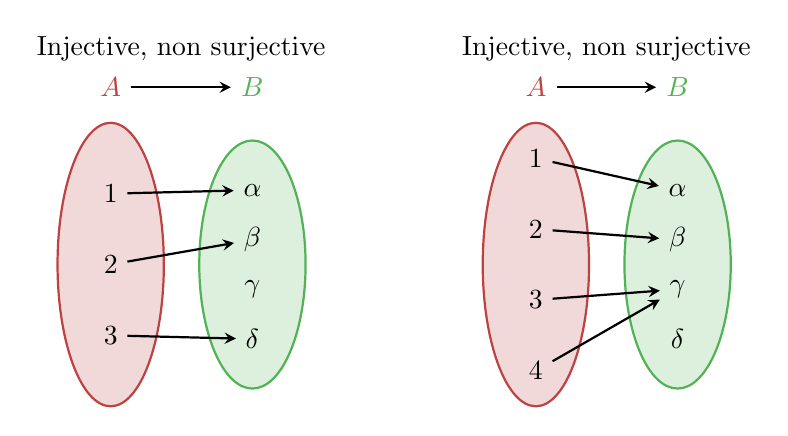
\begin{tikzpicture}[scale=0.9]
		% Injection not surjection
		\fill[xred!20, draw=xred, thick] (0,0) circle (0.75cm and 2cm) node[above, yshift=2cm, text=xred] (A) {$A$};
		\node (A1) at (0,1) {$1$};
		\node (A2) at (0,0)	{$2$};
		\node (A3) at (0,-1) {$3$};

		\fill[xgreen!20, draw=xgreen, thick] (2,0) circle (0.75cm and 1.75cm) node[above, yshift=2cm, text=xgreen] (B) {$B$};
		\node (B1) at (2,1.05) {$\alpha$};
		\node (B2) at (2,0.35) {$\beta$};
		\node (B3) at (2,-0.35) {$\gamma$};
		\node (B3) at (2,-1.05) {$\delta$};

		\draw[arrow] (A1) -- (B1);
		\draw[arrow] (A2) -- (B2);
		\draw[arrow] (A3) -- (B3);

		\draw[arrow] (A) to node[midway, above, yshift=2mm] {Injective, non surjective} (B);
		
		% Surjection not injection
		\fill[xred!20, draw=xred, thick] (6,0) circle (0.75cm and 2cm) node[above, yshift=2cm, text=xred] (A) {$A$};
		\node (A1) at (6,1.5) {$1$};
		\node (A2) at (6,0.5)	{$2$};
		\node (A3) at (6,-0.5) {$3$};
		\node (A4) at (6,-1.5) {$4$};

		\fill[xgreen!20, draw=xgreen, thick] (8,0) circle (0.75cm and 1.75cm) node[above, yshift=2cm, text=xgreen] (B) {$B$};
		\node (B1) at (8,1.05) {$\alpha$};
		\node (B2) at (8,0.35) {$\beta$};
		\node (B3) at (8,-0.35) {$\gamma$};
		\node (B4) at (8,-1.05) {$\delta$};

		\draw[arrow] (A1) -- (B1);
		\draw[arrow] (A2) -- (B2);
		\draw[arrow] (A3) -- (B3);
		\draw[arrow] (A4) -- (B3);

		\draw[arrow] (A) to node[midway, above, yshift=2mm] {Injective, non surjective} (B);
	\end{tikzpicture}

	\vspace{1em}
	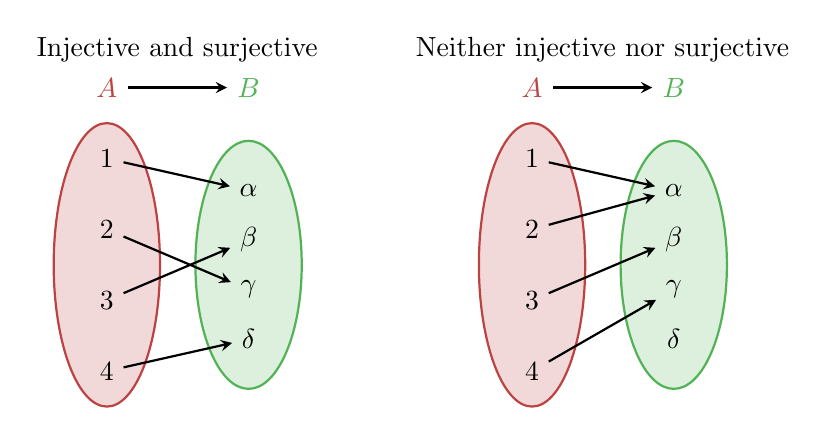
\begin{tikzpicture}[scale=0.9]
		% Injection and surjection
		\fill[xred!20, draw=xred, thick] (0,0) circle (0.75cm and 2cm) node[above, yshift=2cm, text=xred] (A) {$A$};
		\node (A1) at (0,1.5) {$1$};
		\node (A2) at (0,0.5)	{$2$};
		\node (A3) at (0,-0.5) {$3$};
		\node (A4) at (0,-1.5) {$4$};

		\fill[xgreen!20, draw=xgreen, thick] (2,0) circle (0.75cm and 1.75cm) node[above, yshift=2cm, text=xgreen] (B) {$B$};
		\node (B1) at (2,1.05) {$\alpha$};
		\node (B2) at (2,0.35) {$\beta$};
		\node (B3) at (2,-0.35) {$\gamma$};
		\node (B4) at (2,-1.05) {$\delta$};

		\draw[arrow] (A1) -- (B1);
		\draw[arrow] (A2) -- (B3);
		\draw[arrow] (A3) -- (B2);
		\draw[arrow] (A4) -- (B4);

		\draw[arrow] (A) to node[midway, above, yshift=2mm] {Injective and surjective} (B);
		
		% Surjection not injection
		\fill[xred!20, draw=xred, thick] (6,0) circle (0.75cm and 2cm) node[above, yshift=2cm, text=xred] (A) {$A$};
		\node (A1) at (6,1.5) {$1$};
		\node (A2) at (6,0.5)	{$2$};
		\node (A3) at (6,-0.5) {$3$};
		\node (A4) at (6,-1.5) {$4$};

		\fill[xgreen!20, draw=xgreen, thick] (8,0) circle (0.75cm and 1.75cm) node[above, yshift=2cm, text=xgreen] (B) {$B$};
		\node (B1) at (8,1.05) {$\alpha$};
		\node (B2) at (8,0.35) {$\beta$};
		\node (B3) at (8,-0.35) {$\gamma$};
		\node (B4) at (8,-1.05) {$\delta$};

		\draw[arrow] (A1) -- (B1);
		\draw[arrow] (A2) -- (B1);
		\draw[arrow] (A3) -- (B2);
		\draw[arrow] (A4) -- (B3);

		\draw[arrow] (A) to node[midway, above, yshift=2mm] {Neither injective nor surjective} (B);
	\end{tikzpicture}
\end{example}

\vspace{2em}
\begin{note}{Other names for bijections}{bijections}
	Bijections are also called \emph{one-to-one correspondences} and \emph{invertible functions}.
\end{note}

\subsection{Real functions}
In suitable cases, a function is defined via a general mapping rule. This should be very familiar to anyone who learned mathematics in highschool, where many times functions are defined this way, e.g.
\begin{equation}
	f(x) = x^{2}+3x-4.
	\label{eq:function_by_formula}
\end{equation}

In mapping notation we can write \autoref{eq:function_by_formula} as $f:x\mapsto x^{2}+3x-4$. In highschool mathematics, both the domain and image of such functions is $\mathbb{R}$, although it is almost never specified explicitly. Such functions are commonly referred to as \emph{real functions}, a convention used in this book as well.

\begin{example}{Functions defined using a mapping rule}{}
	The following are real functions:
	\[
		f_{1}(x) = 2x^{2}-5,\quad f_{2}(x)=\sin\left( \frac{x}{3} \right),\quad f_{3}(x)=\frac{1}{\sqrt{2\pi}}e^{-\frac{(x-\mu)^{2}}{\sigma^{2}}}.
	\]

	Note that these functions can also be defined using different sets, for example $f_{1}:\mathbb{N}\to\mathbb{Z},\quad f_{2}:\mathbb{N}\to[-1,1],\quad$ etc.
\end{example}

Real functions can be easily plotted in a \emph{Cartesian coordinate system} by drawing all the points $\left( x,f(x) \right)$ (i.e. all the points $\left( x,y \right)$, where $x,y\in\mathbb{R}$ and $x\mapsto y$). We call these points the \emph{graph} of $f$ over $\mathbb{R}$.

\begin{example}{Graphs of real functions}{graph_of_functions}
	The following two functions are plotted on the domain $\left[ -9,9 \right]$:

	\begin{minipage}{0.35\textwidth}
		\begin{itemize}
			\item \textcolor{xred}{$\bm{f(x)=x^{2}-2x-3}$},
			\item \textcolor{xgreen}{$\bm{g(x)=4e^{x}/\left( e^{x}+1 \right)}$}.
		\end{itemize}
	\end{minipage}%
	\begin{minipage}[c]{0.65\textwidth}
		\centering
		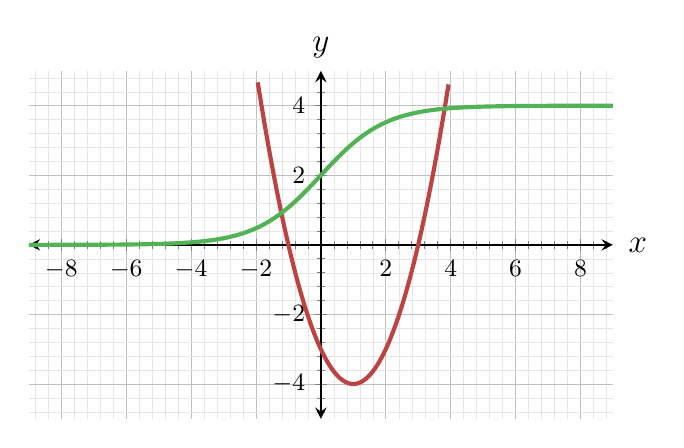
\begin{tikzpicture}
			\begin{axis}[
					graph2d,
					width=9cm, height=6cm,
					xmin=-9, xmax=9,
					ymin=-5, ymax=5,
					domain=-9:9,
					restrict y to domain=-5:5,
					declare function={f(\x)=\x^2-2*\x-3;},
					declare function={g(\x)=4*exp(\x)/(1+exp(\x));},
				]
				\addplot[function, color=xred] {f(x)};
				\addplot[function, color=xgreen] {g(x)};
			\end{axis}
		\end{tikzpicture}
	\end{minipage}
\end{example}

In \autoref{example:graph_of_functions}, the function $g(x)$ always increases in value from left to right. Let's give this notion a more formal tone: a function $f$ is said to be \emph{increasing} on an interval $I$ if for any $x_{1},x_{2}\in I$, if $x_{2}>x_{1}$ then $f\left( x_{2} \right) > f\left( x_{1} \right)$. We can similarily define the idea of \emph{decreasing} on an interval.

A property of some functions which is visually easy to depict is symmetry. A real function $f$ is said to be \emph{symmetric} if for any $x\in\mathbb{R},\ f(-x)=f(x)$. This essentially means that the $y$-axis mirrors the function's plot. If for any $x\in\mathbb{R},\ f(-x)=-f(x)$, we say that the function is \emph{anti-symmetric}. A function can be neither, but there's only a single function which is both: the zero function, i.e. $f(x)=0$.

\begin{example}{Symmetric and anti-symmetric functions}{function_symmetry}
	In the following graphs, the function on the top is symmetric, while the function on the bottom is anti-symmetric:
	\begin{figure}[H]
		\centering
		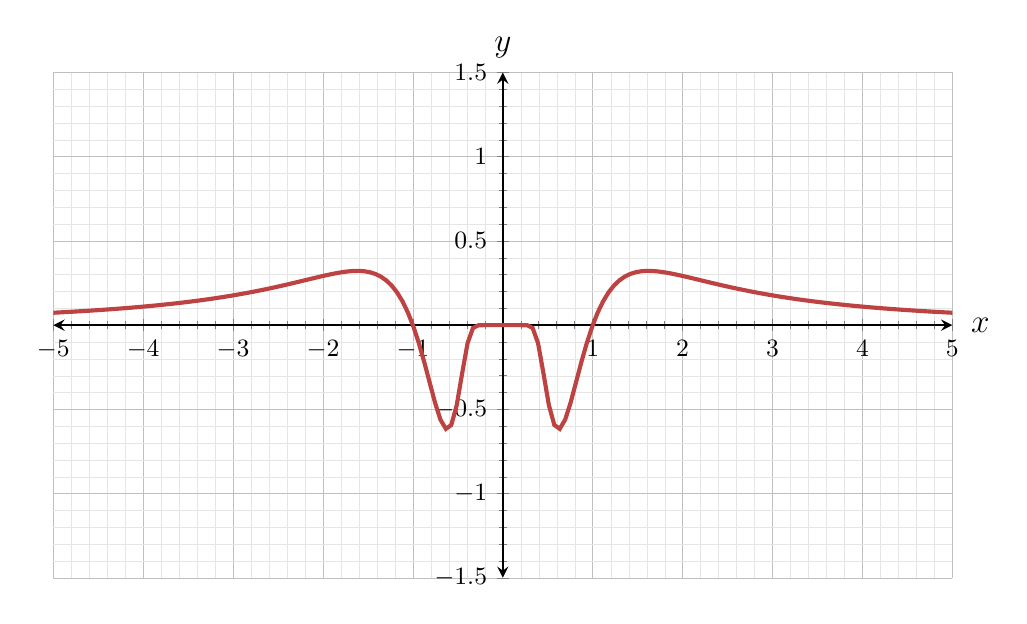
\begin{tikzpicture}
			\begin{axis}[
					graph2d,
					width=13cm, height=8cm,
					xmin=-5, xmax=5,
					ymin=-1.5, ymax=1.5,
					domain=-6:6,
					restrict y to domain=-1.5:1.5,
				]
				\addplot[function, xred] {(2*\x^2-2)*exp(-1/\x^2)/\x^4};
				%\addplot[function, xblue] {(2*\x^2-2)*exp(-1/\x^2)/\x^5};

					%\left(2x^{2}-2\right)\cdot\frac{\exp\left(-\frac{1}{x^{2}}\right)}{x^{4}}
			\end{axis}
		\end{tikzpicture}

		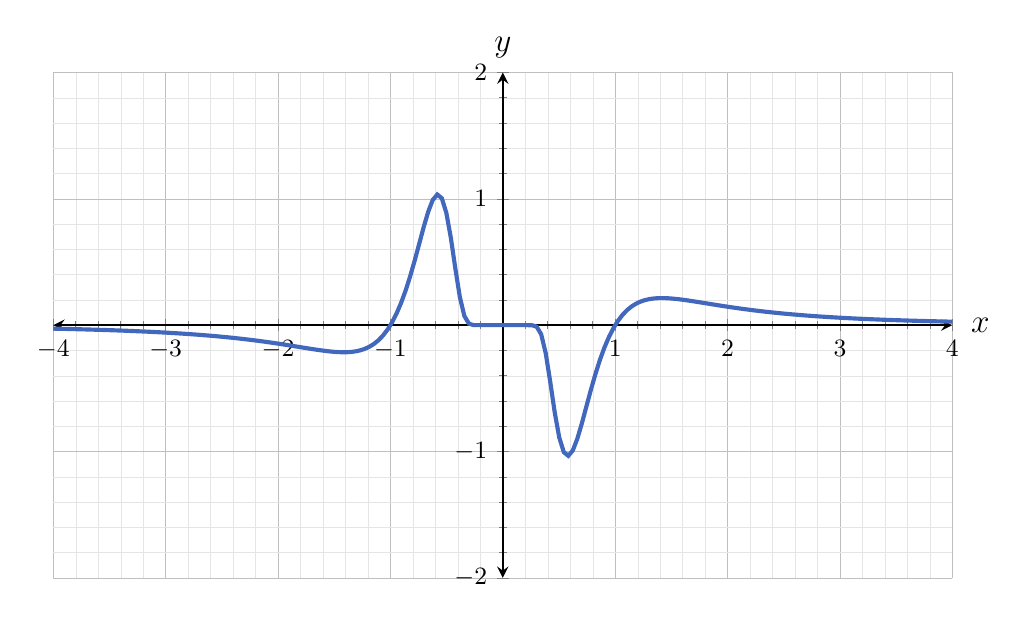
\begin{tikzpicture}
			\begin{axis}[
					graph2d,
					width=13cm, height=8cm,
					xmin=-4, xmax=4,
					ymin=-2, ymax=2,
					domain=-4:4,
					restrict y to domain=-2:2,
				]
				\addplot[function, xblue] {(2*\x^2-2)*exp(-1/\x^2)/\x^5};
			\end{axis}
		\end{tikzpicture}
	\end{figure}
\end{example}

(injections/surjections of real functions?)
 
A real function is said to be \emph{periodic} if it repeats its values exactly over and over with increasing $x$. In more precise terms we define a real function $f$ to be periodic if for any integer value $k$,
\begin{equation}
	f(x+kT) = f(x).
	\label{eq:periodic function}
\end{equation}
where $T=[a,b]$ is a finite interval of $\mathbb{R}$ which we call the \emph{period} of the function.

\begin{example}{A periodic function}{periodic function}
	The following graph depicts a periodic function $f$, with its period $T$ shown. Notice that for any $x\ f(x+T)=f(x)$, i.e. you can move the period measure left and right along the $x$-axis and the values of $f(x)$ in both its edges would always be the equal.

	\centering
	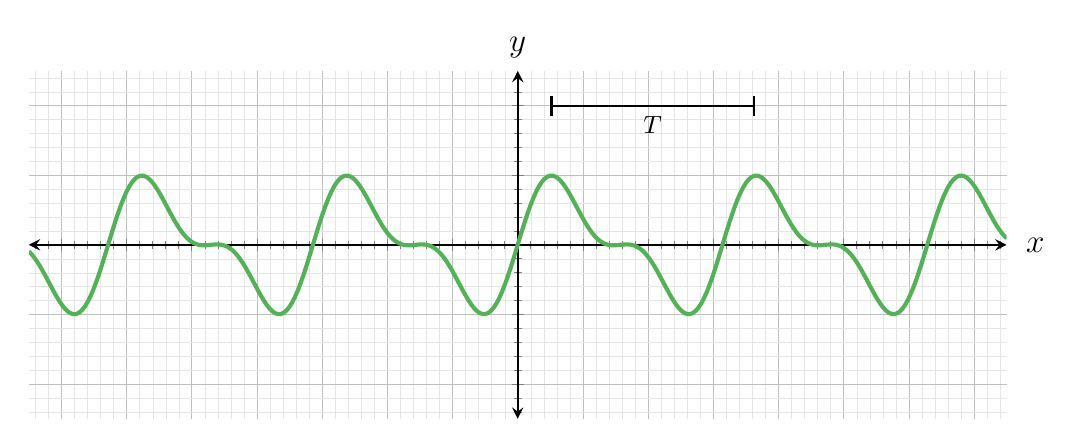
\begin{tikzpicture}
		\begin{axis}[
				graph2d,
				width=14cm, height=6cm,
				xmin=-15, xmax=15,
				ymin=-5, ymax=5,
				xticklabels={},
				yticklabels={},
				domain=-15:15,
				restrict y to domain=-6:6,
				samples=350,
			]
			\addplot[function, xgreen] {0.8*sin(deg(2*\x))+1.5*sin(deg(\x))};
			\draw[|-|, thick] (1,4) -- node[midway, below] {$T$} ({2*pi+1},4);
		\end{axis}
	\end{tikzpicture}
\end{example}

Two additional measures that arise from a period $T$ are the \emph{frequency} $f=\frac{1}{T}$, and the \emph{angular frequency} $\omega=2\pi f=\frac{2\pi}{T}$. We will use these measures later in the book.

\vspace{2em}
\begin{note}{Units of period and frequency}{}
	In a periodic function such as the one in the above example, the units for the period are the same one used for the horizontal axis, while the units of both frequency and angular frequency are both 1 over the unit used for the horizontal axis/period. For example, if the unit of the horizontal axis is that of seconds, then the frequency units are 1/seconds, i.e. Hertz (SI symbol: \si{Hz}).
\end{note}

\subsection{Composition of functions}
Functions can be \emph{composed} together, generating new functions. Given two functions $f:A\to B$ and $g:B\to C$, their composition is denoted as $f\circ g$. For the composition to be well defined, the \textbf{image} of $f$ must be the same as the \textbf{domain} of $g$, and the resulting composition would have $A$ as its domain and $C$ as its image, i.e. $f\circ g:A\to C$.

\begin{example}{Composition of functions}{composition}
	Consider the functions
	\[
		f(x)=x^{2},\quad g(x)=\sin(x).
	\]
	Using these functions, the two possible compositions are
	\begin{itemize}
		\item $f\circ g = f\left( g(x) \right) = \left[ \sin(x) \right]^{2}$, and
		\item $g\circ f = g\left( f(x) \right) = \sin\left( x^{2} \right)$.
	\end{itemize}
\end{example}

\begin{example}{Graphical representation of function composition}{}
	A graphical representation of composing two functions:
	\[
		f:\{1,2,3,4\}\to\{\alpha,\beta,\gamma,\delta\},\quad g:\{\alpha,\beta,\gamma,\delta\}\to\{a,b,c\}.
	\]
	\begin{figure}[H]
		\centering
		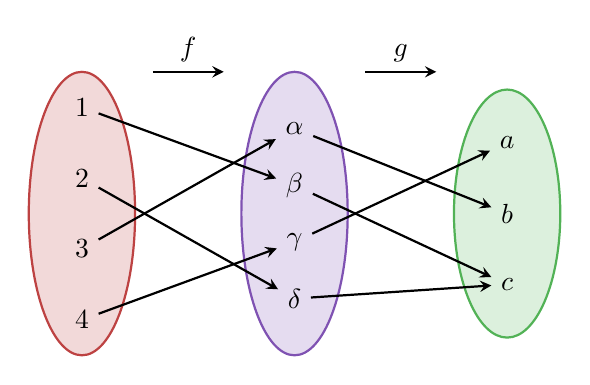
\begin{tikzpicture}[scale=0.9]
			\fill[xred!20, draw=xred, thick] (0,0) circle (0.75cm and 2cm);
			\node (A1) at (0,1.5) {$1$};
			\node (A2) at (0,0.5) {$2$};
			\node (A3) at (0,-0.5) {$3$};
			\node (A4) at (0,-1.5) {$4$};

			\fill[xpurple!20, draw=xpurple, thick] (3,0) circle (0.75cm and 2cm);
			\node (B1) at (3,1.2) {$\alpha$};
			\node (B2) at (3,0.4) {$\beta$};
			\node (B3) at (3,-0.4) {$\gamma$};
			\node (B4) at (3,-1.2) {$\delta$};

			\draw[arrow, thick] (1,2) -- node [midway, above] {$f$} ++(1,0);
			\draw[arrow, thick] (4,2) -- node [midway, above] {$g$} ++(1,0);

			\fill[xgreen!20, draw=xgreen, thick] (6,0) circle (0.75cm and 1.75cm);
			\node (C1) at (6,1) {$a$};
			\node (C2) at (6,0) {$b$};
			\node (C3) at (6,-1) {$c$};

			\draw[arrow] (A1) -- (B2);
			\draw[arrow] (A2) -- (B4);
			\draw[arrow] (A3) -- (B1);
			\draw[arrow] (A4) -- (B3);
			\draw[arrow] (B1) -- (C2);
			\draw[arrow] (B2) -- (C3);
			\draw[arrow] (B3) -- (C1);
			\draw[arrow] (B4) -- (C3);
		\end{tikzpicture}
	\end{figure}
	
	The composition results in the following function
	\[
		f\circ g:\{1,2,3,4\}\to\{a,b,c,\}.
	\]
	\begin{figure}[H]
		\centering
		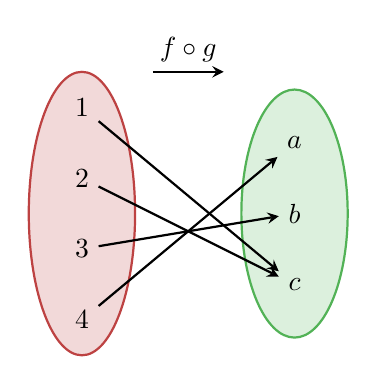
\begin{tikzpicture}[scale=0.9]
			\fill[xred!20, draw=xred, thick] (0,0) circle (0.75cm and 2cm);
			\node (A1) at (0,1.5) {$1$};
			\node (A2) at (0,0.5) {$2$};
			\node (A3) at (0,-0.5) {$3$};
			\node (A4) at (0,-1.5) {$4$};

			\draw[arrow, thick] (1,2) -- node [midway, above] {$f\circ g$} ++(1,0);

			\fill[xgreen!20, draw=xgreen, thick] (3,0) circle (0.75cm and 1.75cm);
			\node (C1) at (3,1) {$a$};
			\node (C2) at (3,0) {$b$};
			\node (C3) at (3,-1) {$c$};

			\draw[arrow] (A1) -- (C3);
			\draw[arrow] (A2) -- (C3);
			\draw[arrow] (A3) -- (C2);
			\draw[arrow] (A4) -- (C1);
		\end{tikzpicture}
	\end{figure}
\end{example}

%\section{Polynomial functions}
A very useful family of real functions can be derived using only three fundamental operations: addition, multiplication and exponentiation: the (real) \emph{polynomial functions}. These are functions of the form
\begin{equation}
	P_{n}(x) = a_{0} + a_{1}x + a_{2}x^{2} + a_{3}x^{3} + \cdots + a_{n}x^{n},
	\label{eq:polynomial_function}
\end{equation}
where $a_{0},a_{1},\dots,a_{n}$ are real numbers called the \emph{coefficients} of the polynomial function. Note that $a_{n}\neq0$, i.e. the \emph{degree} of the polynomial function is the index of the highest non-zero coefficient (and thus the highest power in the expression). We also call this the \emph{order} of the polynomial function.

\begin{example}{Polynomial}{}
	The following is a polynomial function of degree $n=6$:
	\[
		P(x) = 4 + 2x - 3x^{2} + 7x^{4} - x^{5} + 3x^{6}.
	\]

	Breaking down this polynomial to its constituent terms:
	\begin{figure}[H]
		\centering
		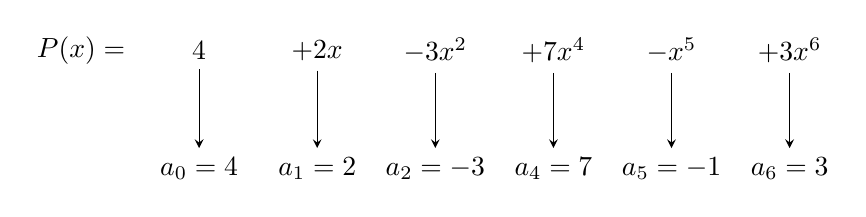
\begin{tikzpicture}[node distance=15mm]
			\node (P) {$P(x)=$};
			\node[right of=P]  (x0) {$4$};
			\node[right of=x0] (x1) {$+2x$};
			\node[right of=x1] (x2) {$-3x^{2}$};
			\node[right of=x2] (x4) {$+7x^{4}$};
			\node[right of=x4] (x5) {$-x^{5}$};
			\node[right of=x5] (x6) {$+3x^{6}$};
			
			\node[below of=x0] (a0) {$a_{0}=4$};
			\node[below of=x1] (a1) {$a_{1}=2$};
			\node[below of=x2] (a2) {$a_{2}=-3$};
			\node[below of=x4] (a4) {$a_{4}=7$};
			\node[below of=x5] (a5) {$a_{5}=-1$};
			\node[below of=x6] (a6) {$a_{6}=3$};

			\draw[arrow, thin] (x0) -- (a0);
			\draw[arrow, thin] (x1) -- (a1);
			\draw[arrow, thin] (x2) -- (a2);
			\draw[arrow, thin] (x4) -- (a4);
			\draw[arrow, thin] (x5) -- (a5);
			\draw[arrow, thin] (x6) -- (a6);
		\end{tikzpicture}
	\end{figure}

	Note that $a_{3}$ is missing from the polynomial function (i.e. there is no $x^{3}$ term). This means that $a_{3}=0$.
\end{example}

A shorthand way to write the general form of a polynomial function is by using the \emph{summation notation}:
\begin{equation}
	P(x) = \sum\limits_{k=0}^{n}a_{k}x^{k}.
	\label{eq:summation_notation}
\end{equation}
This notation, called the \emph{Capital-sigma notation}, essentially represents addition of $n$ elements (in the case shown here), each with its own \emph{index of summation}, in this case $i$. The most general form of the summation notation is
\begin{equation}
	\sum\limits_{i=k}^{n}a_{i} = a_{k} + a_{k+1} + a_{k+2} + \cdots + a_{n-1} + a_{n},
	\label{eq:summation_notation_general}
\end{equation}
i.e. the notation tells us to add those elements $a_{i}$ for which $k\geq i\geq n$. Note that in the case of \autoref{eq:summation_notation}, when $k=0,\ x^{k}=x^{0}=1$ and the first term of the polynomial function has no $x$ power (i.e. it is simply $a_{0}$), and when $k=1,\ x^{k}=x^{1}=x$ and thus the second term is $a_{1}x$. We will encounter the summation notation in more details later in the book.

In the special case $n=0$, i.e. when $P(x)=a_{0}$, the function is constant. When $n=1$ the function $P(x)=a_{0}+a_{1}x$ is a line, and when $n=2,\ P(x)=a_{0}+a_{1}x+a_{2}x^{2}$ is a quadratic function.

\begin{example}{Polynomial functions for $n=0,1,2$}{special_polynomials}
	The following graphs represent the polynomial functions of degrees $n=0,1,2$ with coefficients $a_{0}=2,\ a_{1}=1,\ a_{2}=\frac{1}{2}$:

	\begin{figure}[H]
		\centering
		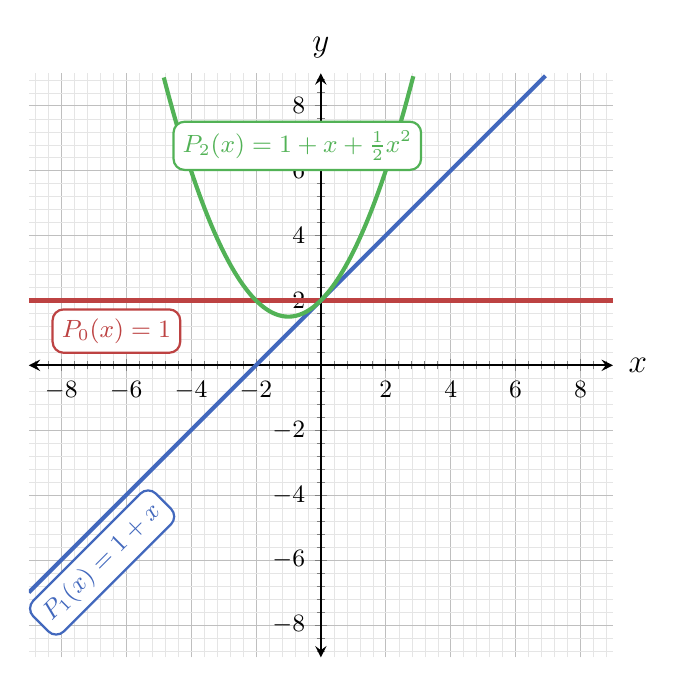
\begin{tikzpicture}
			\tikzset{flbl/.style={draw=#1, thick, fill=white, rounded corners}}
			\begin{axis}[
					graph2d,
					width=9cm, height=9cm,
					xmin=-9, xmax=9,
					ymin=-9, ymax=9,
					domain=-9:9,
					restrict y to domain=-9:9,
					declare function={p0(\x)=2;},
					declare function={p1(\x)=2+\x;},
					declare function={p2(\x)=2+\x+0.5*\x^2;},
				]
				\addplot[function, xred] {p0(x)} node[flbl=xred, below, pos=0.15, yshift=-1mm] {$P_{0}(x)=1$};
				\addplot[function, xblue] {p1(x)} node[flbl=xblue, below, pos=0.1, rotate=45, yshift=-1mm] {$P_{1}(x)=1+x$};
				\addplot[function, xgreen] {p2(x)} node[flbl=xgreen, right, pos=0.2, xshift=-3mm, yshift=5mm] {$P_{2}(x)=1+x+\frac{1}{2}x^{2}$};
			\end{axis}
		\end{tikzpicture}
	\end{figure}
\end{example}

The values $x\in\mathbb{R}$ for which $P(x)=0$ are called the \emph{roots} (also: \emph{zeros}) of the polynomial function.

\begin{example}{Roots of a polynomial function}{}
	The polynomial function $P(x) = 24x - 50x^{2} + 35x^{3} - 10x^{4} + x^{5}$ has the following $5$ roots: $x_{0}=0,\ x_{1}=1,\ x_{2}=2,\ x_{3}=3,\ x_{4}=4$. In the following graph of $P(x)$ the roots are shown as black dots.
	\begin{figure}[H]
		\centering
		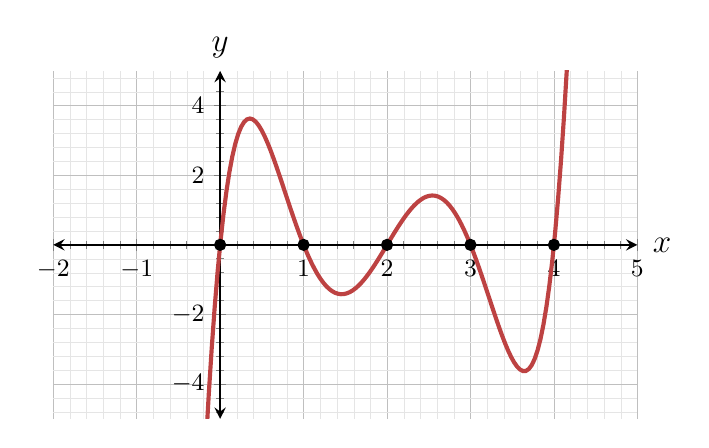
\begin{tikzpicture}
			\begin{axis}[
					graph2d,
					width=9cm, height=6cm,
					xmin=-2, xmax=5,
					ymin=-5, ymax=5,
					domain=-2:5,
					restrict y to domain=-6:6,
					declare function={P(\x)=\x*(\x-1)*(\x-2)*(\x-3)*(\x-4);},
				]
				\addplot[function, xred] {P(x)};
				\addplot[black, only marks, mark=*, samples at={0,1,...,4}] {P(x)};
			\end{axis}
		\end{tikzpicture}
	\end{figure}
\end{example}

The maximum number of \textbf{real} roots of a polynomial function with degree $n\geq1$ is $n$, e.g. a polynomial of degree $n=4$ has at most $4$ real roots. This statement is a consequence of a very important theorem called \emph{the fundamental theorem of algebra}, which due to its importance we will mention here without proof:

\begin{theorem}{The fundamental theorem of algebra}{fundamental}
	For any $n\geq1$, the polynomial function $P(z)=a_{0}+a_{1}z+a_{2}z^{2}+\cdots+a_{n}z^{n}$, where $a_{0},a_{1},a_{2},\dots,a_{n}$ are all \textbf{complex numbers} and $a_{n}\neq0$, has $n$ complex roots.
\end{theorem}

Given a polynomial function $P(x)$ with $n$ roots $r_{1},\ r_{2},\ \cdots,\ r_{n}$, the function can be written as a product of terms of the form $x-r_{i}$ (up to a constant), e.g. the polynomial function of degree $n=3$ with roots $-1,1,2$ can be written as
\begin{equation}
	P(x) = (x+1)(x-1)(x-2) = x^{3}-2x^{2}-x+2.
	\label{eq:roots_form}
\end{equation}

\begin{example}{Higher order polynomial functions}{high_order_polynomials}
	The following are the graphs of high-order polynomial functions ($n=3,4,5,6$):

	\begin{figure}[H]
		\captionsetup[subfigure]{labelformat=empty}
		\centering
		\begin{subfigure}[b]{0.475\textwidth}
			\centering
			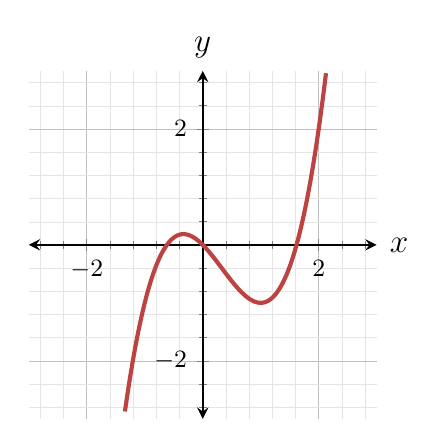
\begin{tikzpicture}
				\begin{axis}[
						graph2d,
						width=6cm, height=6cm,
						xmin=-3, xmax=3,
						ymin=-3, ymax=3,
						domain=-3:3,
						restrict y to domain=-3:3,
						declare function={P3(\x)=\x^3-\x^2-\x;},
					]
					\addplot[function, xred] {P3(x)};
				\end{axis}
			\end{tikzpicture}
			\caption{\textcolor{xred}{$\bm{x^{3}-x^{2}-x}$}}
		\end{subfigure}
		\hfill
		\begin{subfigure}[b]{0.475\textwidth}
			\centering
			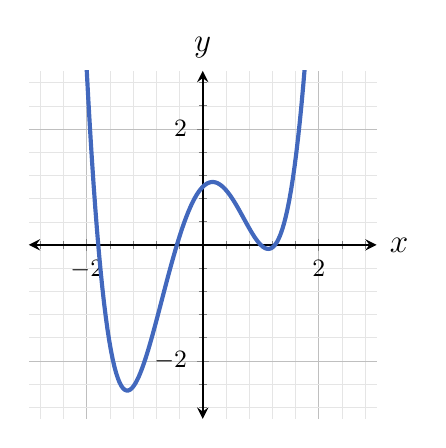
\begin{tikzpicture}
				\begin{axis}[
						graph2d,
						width=6cm, height=6cm,
						xmin=-3, xmax=3,
						ymin=-3, ymax=3,
						domain=-3:3,
						restrict y to domain=-10:10,
						declare function={P4(\x)=\x^4-3*\x^2+\x+1;},
					]
					\addplot[function, xblue] {P4(x)};
				\end{axis}
			\end{tikzpicture}
			\caption{\textcolor{xblue}{$\bm{x^{4}-3x^{2}+x+1}$}}
		\end{subfigure}

		\begin{subfigure}[b]{0.475\textwidth}
			\centering
			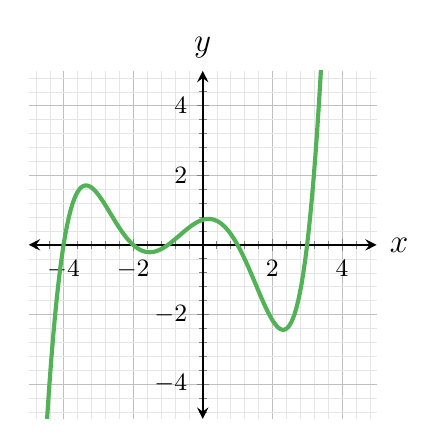
\begin{tikzpicture}
				\begin{axis}[
						graph2d,
						width=6cm, height=6cm,
						xmin=-5, xmax=5,
						ymin=-5, ymax=5,
						domain=-5:5,
						restrict y to domain=-10:10,
						declare function={P5(\x)=0.03*(\x^5+3*\x^4-11*\x^3-27*\x^2+10*\x+24);},
					]
					\addplot[function, xgreen] {P5(x)};
				\end{axis}
			\end{tikzpicture}
			\caption{\textcolor{xgreen}{$\bm{\frac{3}{100}\left( x^{5}+3x^{4}-11x^{3}-27x^{2}+10x+24 \right)}$}}
		\end{subfigure}
		\hfill
		\begin{subfigure}[b]{0.475\textwidth}
			\centering
			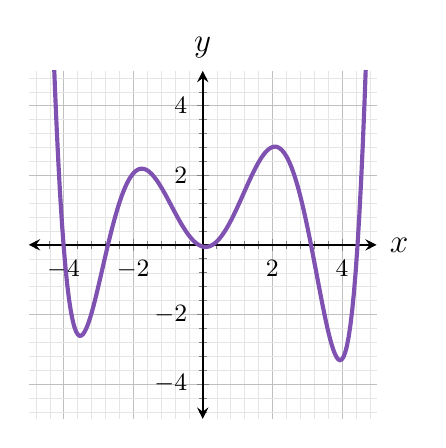
\begin{tikzpicture}
				\begin{axis}[
						graph2d,
						width=6cm, height=6cm,
						xmin=-5, xmax=5,
						ymin=-5, ymax=5,
						domain=-5:5,
						restrict y to domain=-15:15,
						declare function={P6(\x)=0.01*(x^6-x^5-26*x^4+15*x^3+150*x^2-25*x-5);},
					]
					\addplot[function, xpurple] {P6(x)};
				\end{axis}
			\end{tikzpicture}
			\caption{\textcolor{xpurple}{$\bm{\frac{1}{100}\left( x^{6}-x^{5}-26x^{4}+15x^{3}+150x^{2}-25x-5\right)}$}}
		\end{subfigure}
	\end{figure}
\end{example}

As can be seen in \autoref{:high_order_polynomials}, the maximal number of `bends' in a polynomial function of order $n$ is $n-1$ (i.e. one less than the order of the function).

We will continue to explore polynomial functions in more details in future chapters.

%\section{Exponential and Logarithmic Functions}
In the previous section we dealt with functions composed of integer powers of $x$. We will now shortly focus on functions where $x$ is in the power itself and their inverse functions.

An \emph{exponential function}, or simply an \emph{exponential}, is a real function of the type
\begin{equation}
	f(x) = b^{x},
	\label{eq:exponent}
\end{equation}
where $b>0$ is called the \emph{base} of the exponentiation, and $x$ the exponential. All exponents, regardless of base, are always positive. In addition, all exponents pass through the point $(0,1)$ since $b^{0}=1$ for any real positive number, and through the point $(1,b)$ since $b^{1}=b$. When $b>1$ the function is increasing on $\mathbb{R}$, while for $b<1$ the function is descending on $\mathbb{R}$.

\begin{example}{Exponential functions}{exponents}
	The following are graphs of the exponential functions \textcolor{xred}{$\bm{1.5^{x}}$}, \textcolor{xblue}{$\bm{2^{x}}$} and \textcolor{xgreen}{$\bm{3.5^{x}}$}:
	\begin{figure}[H]
		\centering
		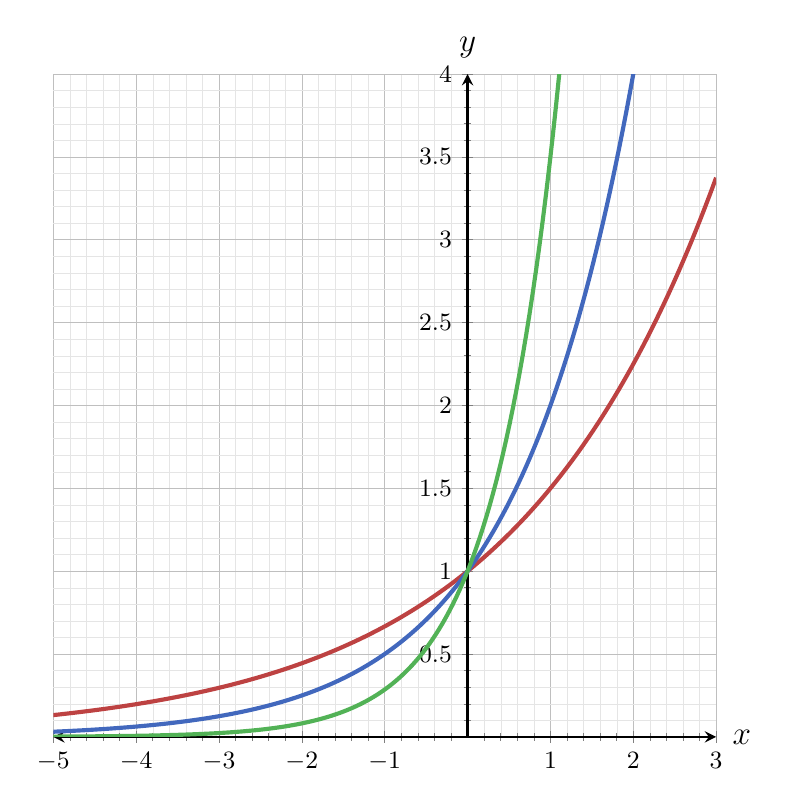
\begin{tikzpicture}
			\begin{axis}[
					graph2d,
					y axis line style={-stealth, thick},
					width=10cm, height=10cm,
					xmin=-5, xmax=3,
					ymin=0, ymax=4,
					domain=-5:3,
					restrict y to domain=0:5,
				]
				\addplot[function, xred] {(1.5)^\x};
				\addplot[function, xblue] {2^\x};
				\addplot[function, xgreen] {3.5^\x};
			\end{axis}
		\end{tikzpicture}
	\end{figure}

	And the following are graphs of the exponential functions \textcolor{xpurple}{$\bm{0.7^{x}}$}, \textcolor{xorange}{$\bm{0.5^{x}}$} and $\bm{0.2^{x}}$:
	\begin{figure}[H]
		\centering
		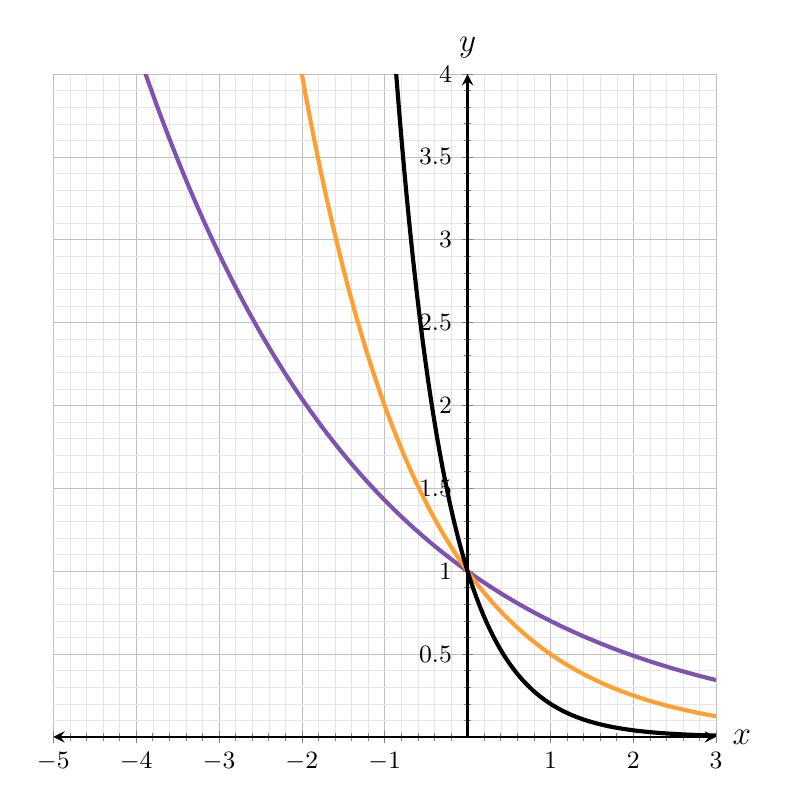
\begin{tikzpicture}
			\begin{axis}[
					graph2d,
					y axis line style={-stealth, thick},
					width=10cm, height=10cm,
					xmin=-5, xmax=3,
					ymin=0, ymax=4,
					domain=-5:3,
					restrict y to domain=0:5,
				]
				\addplot[function, xpurple] {0.7^\x};
				\addplot[function, xorange] {0.5^\x};
				\addplot[function, black] {0.2^\x};
			\end{axis}
		\end{tikzpicture}
	\end{figure}
\end{example}

As a reminder, the following are two well known properties of exponents: given a base $b>0$,
\begin{align}
	b^{-x} &= \frac{1}{b^{x}},\\
	b^{x}b^{y} &= b^{x+y}.
	\label{eq:exponents_properties}
\end{align}

A special base for exponential functions is the real, non-aglebric number $e$. This number has many names, among them is \emph{Euler's number}, but in the constant of exponentials it is known as the \emph{natural base}. Its exact value is not entirely important for the moment: it is about $2.718$, and in any case it is not possible to write it as there it has infinitely many digits after the period. It is very common across different fields of mathematics and science to write $\exp(x)$ instead of $e^{x}$.

The inverse function to exponentials are the \emph{logatithmic functions} (or simply \emph{logarithms}), i.e.\ for any real $b>0,\ b\neq1$,
\begin{equation}
	\log_{b}\left( b^{x} \right) = b^{\log_{b}(x)} = x.
	\label{eq:logarithms}
\end{equation}
In essence, the logarithm in base $b$ of a number $x$ answers the question \textit{``what is the number $a$ for which $b^{a}=x$?''}. Being the inverses of exponential functions, all logarithms go through the point $(1,0)$, and each also passes through its own point $(b,1)$.

\begin{example}{Logarighmic functions}{logarithms}
	The following are graphs of the logatithmic functions \textcolor{xred}{${\log_{1.5}(x)}$}, \textcolor{xblue}{${\log_{2}(x)}$} and \textcolor{xgreen}{${\log_{3.5}(x)}$}:
	\begin{figure}[H]
		\centering
		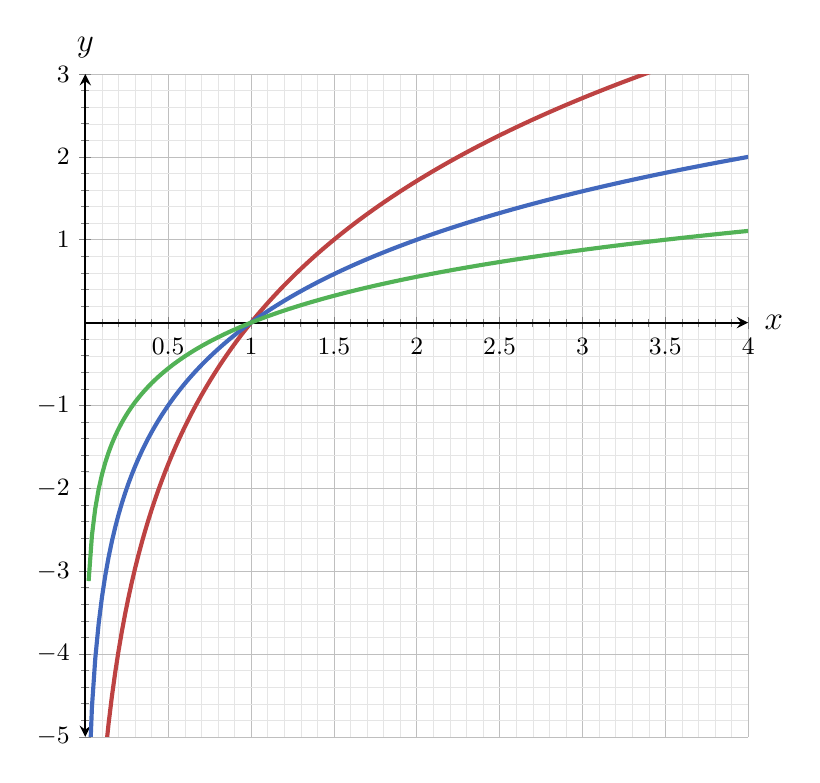
\begin{tikzpicture}
			\begin{axis}[
					graph2d,
					x axis line style={-stealth, thick},
					width=10cm, height=10cm,
					xmin=0, xmax=4,
					ymin=-5, ymax=3,
					domain=0:4,
					restrict y to domain=-10:4,
				]
				\addplot[function, xred] {ln(\x)/ln(1.5)};
				\addplot[function, xblue] {ln(\x)/ln(2)};
				\addplot[function, xgreen] {ln(\x)/ln(3.5)};
			\end{axis}
		\end{tikzpicture}
	\end{figure}

	...and the following are graphs of the exponential functions \textcolor{xpurple}{$\log_{0.75}(x)$}, \textcolor{xorange}{$\log_{0.5}(x)$} and $\log_{0.2}(x)$:
	\begin{figure}[H]
		\centering
		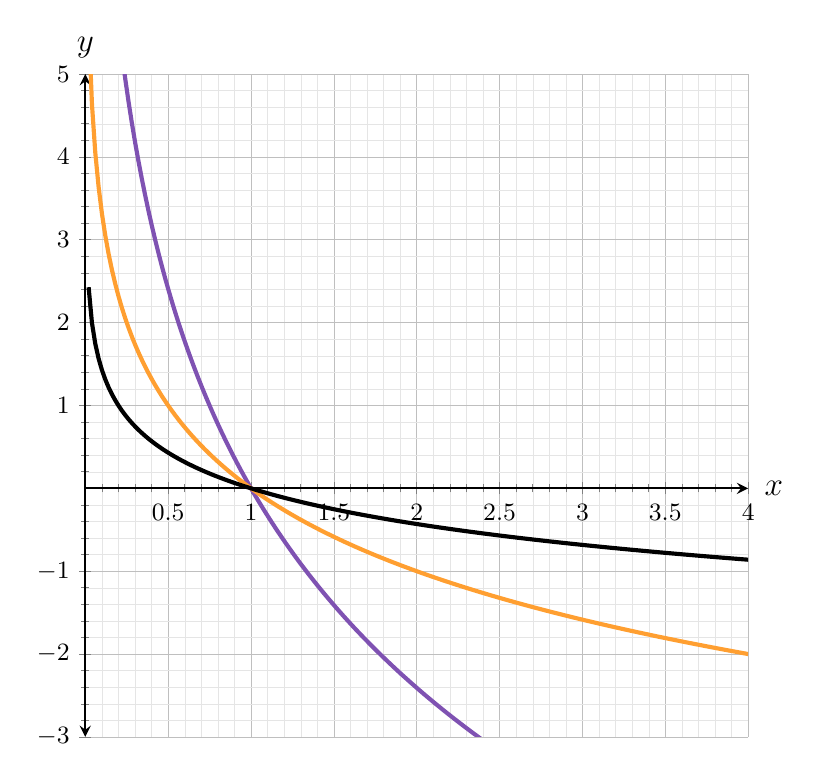
\begin{tikzpicture}
			\begin{axis}[
					graph2d,
					x axis line style={-stealth, thick},
					width=10cm, height=10cm,
					xmin=0, xmax=4,
					ymin=-3, ymax=5,
					domain=0:4,
					restrict y to domain=-4:10,
				]
				\addplot[function, xpurple] {ln(\x)/ln(0.75)};
				\addplot[function, xorange] {ln(\x)/ln(0.5)};
				\addplot[function, black] {ln(\x)/ln(0.2)};
			\end{axis}
		\end{tikzpicture}
	\end{figure}
\end{example}

A useful property of logarithms is that they can help reduce ranges spanning several orders of magnitude to numebrs humans can deal with. The easiest way to see this is using $b=10$: $10^{1}=10$, and so $\log_{10}(10)=1$. $10^{2}=100$, and so $\log_{10}(100)=2$. $10^{3}=1000$, and so $\log_{10}(1000)=3$, etc. The value of the logarithm goes by $1$ for each raise in order of magnitude of its argument.

Therefore, if we have some measurement $x$ which can hold values spanning severl orders of magnitude (say $x\in[3,1500000000]$), then it can sometimes be useful to use instead the logarithmic value of $x$ (which in our case would span the range $\log_{10}(x)\in[0.477,9.176]$). This is done in many fields of science, for example some definitions of entropy\footnote{$S=k_{\text{B}}\log\left( \Omega \right)$}, acid disociation constants\footnote{$\text{p}K_{a}=-\log\left( K_{\text{diss}} \right)$}, pH\footnote{$\text{pH}=-\log\left(\ce{[H+]}\right)$} and more.

\begin{example}{Logarithms as eavluating orders of magnitude}{}
	In the following graph of $\log_{2}(x)$, each increase by power of two in $x$ (i.e. $x=1,2,4,8,16,\dots$) yields only a single increase in $y$ (i.e. $y=0,1,2,3,4,\dots$). This shows how logarithms shift our perspective from absolute values to orders of magnitude.
	\begin{figure}[H]
		\centering
		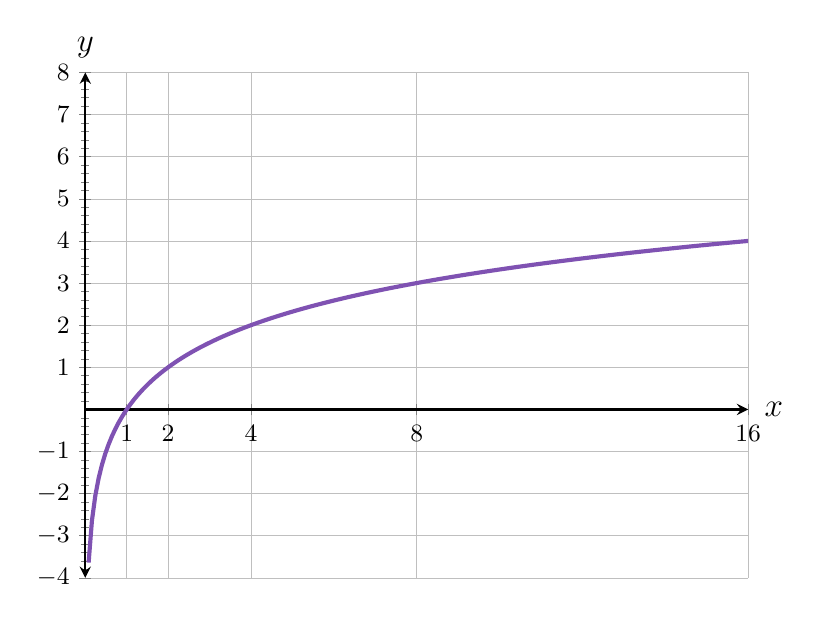
\begin{tikzpicture}
			\begin{axis}[
					graph2d,
					x axis line style={-stealth, thick},
					width=10cm, height=8cm,
					xmin=0, xmax=16,
					ymin=-4, ymax=8,
					domain=0:16,
					restrict y to domain=-7:10,
					grid=major,
					xtick={0,1,2,4,8,16},
					ytick={-4,-3,...,8},
				]
				\addplot[function, xpurple] {ln(\x)/ln(2)};
			\end{axis}
		\end{tikzpicture}
	\end{figure}
\end{example}

Using the definition of the logarithmic function $\log_{b}(x)$ (\eqref{logarithms}) and the product rule for exponentials (\eqref{exponents_properties}), a similar rule can be derived for logarithms. Let $x,y>0$ and $b>0,\ b\neq1$ all be real numbers. We define
\begin{equation}
	\log_{b}(x)=M,\ \log_{b}(y)=N,
	\label{eq:log_addition_rule_step1}
\end{equation}
which means
\begin{equation}
	b^{M}=x,\ b^{N}=y.
	\label{eq:log_addition_rule_step2}
\end{equation}
From \eqref{exponents_properties} we know that
\begin{equation}
	xy = b^{M}b^{N} = b^{M+N},
	\label{eq:log_addition_rule_step3}
\end{equation}
and by re-applying the definition of logarithmic functions we get that
\begin{equation}
	\log_{b}(xy) = M+N = \log_{b}(x) + \log_{b}(y).
	\label{eq:log_addition_rule_step4}
\end{equation}

Simlilarily to \eqref{log_addition_rule_step4}, division yields subtraction:
\begin{equation}
	\log_{b}\left(\frac{x}{y}\right) = \log_{b}(x)-\log_{b}(y).
	\label{eq:log_subtraction_rule}
\end{equation}

Equations \ref{eq:log_addition_rule_step4} and \ref{eq:log_subtraction_rule} reveal another valueable property of logarithms: they reduce multiplication to addition (and subsequently division to subtraction). While today this property doesn't seem very impressive, in pre-computers days it helped carrying on complicated calculations, using tables of pre-calculated logarithms (called simply \emph{logarithm tables}) - a sight rarely seen today.

Taking one step forward in regards to reduction of operations, logarithms reduce powers to multiplication:
\begin{equation}
	\log_{b}\left( x^{k} \right) = k\log_{b}(x).
	\label{eq:log_product_rule}
\end{equation}
for any $k\in\mathbb{R}$.

(TBW:\@ proving this will be in the chapter questions to the reader)

Any logarithm $\log_{b}(x)$ can be expressed using another base, i.e. $\log_{a}(x)$ (where $a>0,\ a\neq1$) using the following formula:
\begin{equation}
	\log_{a}(x) = \log_{b}(x)\cdot\log_{a}(b).
	\label{eq:log_base_change}
\end{equation}
(TBW:\@ proving this too will be a question to the reader)

\begin{example}{Changing logarithm base}{}
	Expressing $\log_{4}(x)$ in terms of $\log_{2}(x)$:
	\[
		\log_{4}(x) = \log_{2}(x)\cdot\underbrace{\log_{4}(2)}_{=\frac{1}{2}} = \frac{1}{2}\log_{2}(x).
	\]
\end{example}

Much like with exponentials, the number $e$ plays an important role when it comes to logarithms, for reasons that are discussed in the calculus chapter (ref). For now, we will just mention that $\log_{e}(x)$ gets a special notation: $\ln(x)$, which stands for \emph{natural logarithm}. This notation is mainly used in applied mathematics and science, while in pure mathematics the notation is simply $\log(x)$, i.e. without mentioning the base \footnote{Depending on convention and context, this notation can refer to logarithm in any other base, most commonly $\log_{10}(x)$ and $\log_{2}(x)$.}.

For reason we will see in the calculus chapter, it is relatively simple to calculate both the exponential and logarithm in base $e$. Therefore, many operations in modern computations are actually done using these functions, for example calculating logarithms in other bases:
\begin{equation}
	\log_{b}(x) = \frac{\ln(x)}{\ln(b)}.
	\label{eq:ln_base_change}
\end{equation}
Another operation commonly using both $e^{x}$ and $\ln(x)$ is raising a real number $a$ to a real power $b$: using the properties of both exponential and logarithmic functions, any such power can be expressed as
\begin{equation}
	a^{b} = e^{b\ln(a)}.
	\label{eq:powers_using_e}
\end{equation}

%\pgfplotsset{
  layers/axis lines on top/.define layer set={
    axis background,
    axis grid,
    axis ticks,
    axis tick labels,
    pre main,
    main,
    axis lines,
    axis descriptions,
    axis foreground,
  }{/pgfplots/layers/standard},
}

\pgfkeys{
	/pgfplots/unit circle/.style={
		set layers=axis lines on top,
		width=9cm, height=9cm,
		axis x line=middle,
		axis y line=middle,
		xlabel=$x$,
		ylabel=$y$,
		every axis x label/.style={
			at={(ticklabel* cs:1.01)},
			anchor=west,
		},
		every axis y label/.style={
			at={(ticklabel* cs:1.01)},
			anchor=south,
		},
		axis line style={stealth-stealth, thick},
		label style={font=\Large},
		tick label style={font=\Large},
		samples=100,
		xmin=-1.25, xmax=1.25,
		ymin=-1.25, ymax=1.25,
		xtick={-1,0,1},
		ytick={-1,0,1},
		xticklabels={},
		yticklabels={},
		domain=-1.5:1.5,
		grid=both,
		major grid style={black!5},
	},
}

\section{Trigonometric functions} % (fold)
\label{sec:trigonometry}

% section section name (end)
\subsection{Basic Definitions}
Consider a \emph{right triangle} $\triangle ABC$ with sides $a,b$, and Hypotenuse $c$, where the angle $\angle ACB$ is $\ang{90}$, and the angle $\angle BAC$ is denoted as $\alpha$:

\centering
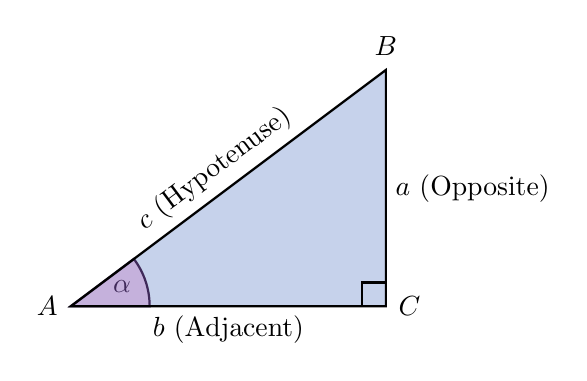
\begin{tikzpicture}[node distance=3mm]
		\coordinate (A) at (0,0);
		\coordinate (B) at (4,3);
		\coordinate (C) at (4,0);

		\node[left of=A] {$A$};
		\node[above of=B] {$B$};
		\node[right of=C] {$C$};

		\draw[fill=xblue!30] (A) -- node (c) [midway, above, rotate=36.87] {$c$ (Hypotenuse)} (B) -- node (a) [midway, right] {$a$ (Opposite)} (C) -- node (b) [midway, below] {$b$ (Adjacent)} cycle;
		\draw[thick] ($(C)+(0,0.3)$) rectangle ($(C)-(0.3,0)$);
		\draw[thick, xpurple!50!black, fill=xpurple!45] (A) -- ($(A)+(1,0)$) arc (0:36.87:1) node [midway, xshift=-3mm, yshift=-2pt] {$\alpha$} -- cycle;
		%\draw[thick, xblue!50!black, fill=xblue!45] (B) -- ($(B)+(0,-0.8)$) arc (270:216.97:0.8) node [midway, above, xshift=5pt] {$\beta$} -- cycle;
		\draw[thick] (A) -- (B) -- (C) -- cycle;
	\end{tikzpicture}
\flushleft

We use the ratios between the three sides of the triangle to define three functions of $\alpha$:
\vspace{5mm}
\begin{itemize}
	\item The \emph{sine} of the angle $\alpha$ is $\sin(\alpha)=\frac{a}{c}$,
	\item the \emph{cosine} of the angle $\alpha$ is $\cos(\alpha)=\frac{b}{c}$, and
	\item the \emph{tangent} of the angle $\alpha$ is $\tan(\alpha)=\frac{a}{b}$, which in turn is equal to $\frac{\sin(\alpha)}{\cos(\alpha)}$.
\end{itemize}

We can rearrange the above definitions:
\begin{align}
	a &= c\sin(\alpha),\nonumber\\
	b &= c\cos(\alpha).
	\label{eq:basic_trig_rearrange}
\end{align}

Normally, the Hypotenuse is the longest side of a right triangle. We will consider here the two edge cases where one of the sides $a$ or $b$ is equal to the Hypotenuse (and the other side is thus $0$):
\begin{itemize}
	\item if $a=c$ then $\alpha=\ang{90}$,\
	\item if $b=c$ then $\alpha=\ang{0}$.
\end{itemize}

The possible length of $a$ is therefore in the range $0\leq a \leq c$, which means that $0\leq \frac{a}{c} \leq 1$. Since $\sin(\alpha)=\frac{a}{c}$ this means that the image of $\sin(\alpha)$ is $[0,1]$. The same idea is also true for $b$, and therefore $[0,1]$ is the image of $\cos(\alpha)$ as well.

As a reminder, the \emph{Pythagorean theorem}\footnote{It's worth mentioning that no three positive integers $a, b$, and $c$ satisfy the equation $a^{n}+b^{n}=c^{n}$ for any integer value of $n>2$. \href{https://en.wikipedia.org/wiki/Fermat\%27s_Last_Theorem}{This can be proven, however the proof is too large to fit in the footnotes}.} states that for a right triangle with sides $a, b$ and $c$,
\begin{equation}
	a^{2} + b^{2} = c^{2}.
	\label{eq:pythagorean_theorem}
\end{equation}
By substituting \xref[eq]{basic_trig_rearrange} into the Pythagorean theorem we get
\begin{align*}
	c^{2} &= a^{2}+b^{2}\\
	&= \left[ c\sin(\alpha) \right]^{2} + \left[ c\cos(\alpha) \right]^{2}\\
	&= c^{2}\sin^{2}(\alpha) + c^{2}\cos^{2}(\alpha)\\
	&= c^{2}\left[ \sin^{2}(\alpha) + \cos^{2}(\alpha) \right],
\end{align*}
and therefore
\begin{equation}
	\sin^{2}(x) + \cos^{2}(x) = 1.
	\label{eq:sin sqr plus cos sqr equals 1}
\end{equation}

\subsection{The Unit Circle}
We defined $\sin(\alpha)$ and $\cos(\alpha)$ so far in way such that their domains are both $[\ang{0},\ang{90}]$, and their images are both $[0,1]$. However, there is a simple way to extend these functions such that both their domains are $\mathbb{R}$, and both their images are $[-1,1]$: by using a \emph{unit circle}.

\autoref{fig:unit_circle} depicts a unit circle: it is simply a circle of radius $R=1$, which is placed such that its center lies at the origin of a 2-dimensional axis system (i.e. at the point $\bm{O}=(0,0)$. We then draw a line from $\bm{O}$ to a point $\bm{P}=(x,y)$ on the circumference of the unit circle. We call the angle between the line $\bm{OP}$ and the $x$-axis $\theta$. We then draw another line, this time from the point $\bm{P}$ to a point $\bm{D}$ on the $x$-axis, such that $\bm{PD}$ is perpendicular to the $x$-axis.

The triangle $\triangle OPD$ is a right triangle. Therefore, we can use the trigonometric functions to calculate the coordinates of the point $\bm{P}=(x,y)$:
\begin{align}
	x &= R\cos(\theta) = \cos(\theta),\nonumber\\
	y &= R\sin(\theta) = \sin(\theta).
	\label{eq:xy_P}
\end{align}

We then define $\cos(\theta)$ and $\sin(\theta)$ as a function of $\theta$:
\begin{align}
	\sin(\theta) &= y,\nonumber\\
	\cos(\theta) &= x.
	\label{eq:unit circle definition of sin and cos}
\end{align}

Using this definition, the angle $\theta$ can take any value between $\ang{0}$ and $\ang{360}$. In fact, the values of $\theta$ can be extended to any real number in degrees: any real value of degrees is equivalent to some value in the range $[\ang{0},\ang{360}]$, the first and most obvious example is that $\ang{360}$ is equivalent to $\ang{0}$. Similarly, $\ang{-30}\equiv\ang{330}$, $-\ang{180}\equiv\ang{180}$, $-\ang{90}\equiv\ang{270}$, etc (see \autoref{fig:angles equivalency}). In fact, this property makes the trigonometric functions periodic, with a period $T=\ang{360}$.

\begin{figure}
	\centering
	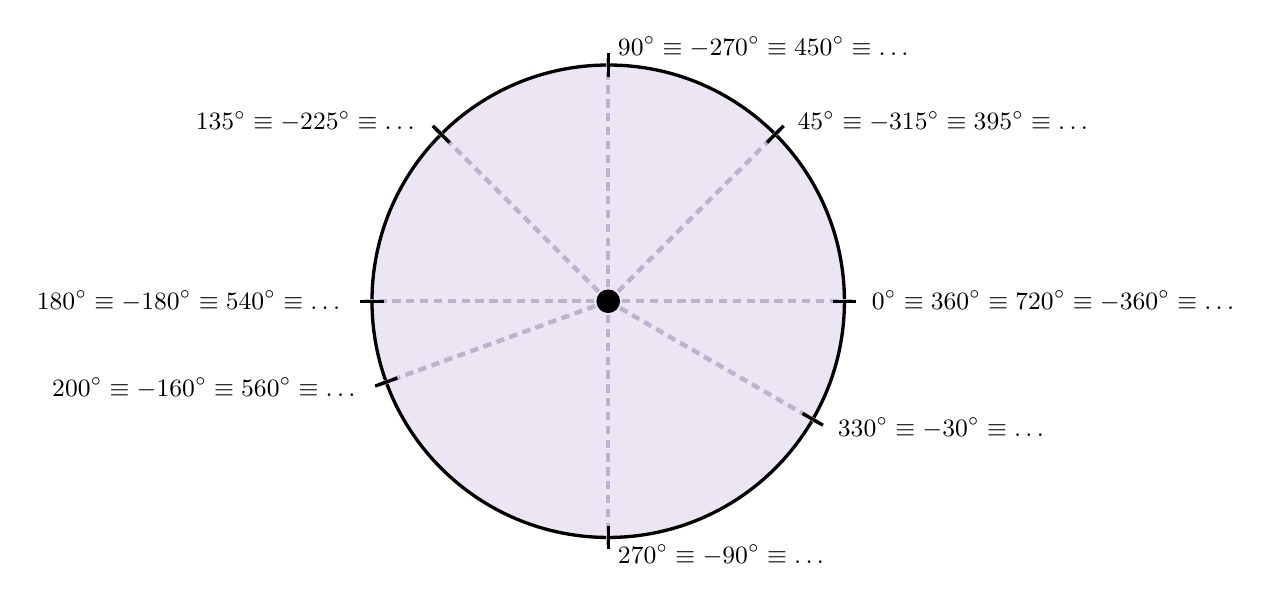
\begin{tikzpicture}[every node/.style={font=\small}]
		\def\R{3}
		\draw[very thick, fill=xpurple!15] (0,0) circle (\R);
		\foreach \th in {0, 45, 90, 135, 180, 200, 270, 330}{
			\draw[ultra thick, densely dashed, xpurple!75!black!40] (0,0) -- ({1.05*\R*cos(\th)},{1.05*\R*sin(\th)});
			\draw[very thick] ({0.95*\R*cos(\th)},{0.95*\R*sin(\th)}) -- ({1.05*\R*cos(\th)},{1.05*\R*sin(\th)});
			\node at ({1.075*\R*cos(\th)},{1.075*\R*sin(\th)}) (\th) {};
		}
		\fill[black] (0,0) circle (0.15);
		\node[right] at (0) {$\ang{0}\equiv\ang{360}\equiv\ang{720}\equiv\ang{-360}\equiv\dots$};
		\node[right] at (45) {$\ang{45}\equiv\ang{-315}\equiv\ang{395}\equiv\dots$};
		\node[right] at (90) {$\ang{90}\equiv\ang{-270}\equiv\ang{450}\equiv\dots$};
		\node[left] at (135) {$\ang{135}\equiv\ang{-225}\equiv\dots$};
		\node[left] at (180) {$\ang{180}\equiv\ang{-180}\equiv\ang{540}\equiv\dots$};
		\node[left] at (200) {$\ang{200}\equiv\ang{-160}\equiv\ang{560}\equiv\dots$};
		\node[right] at (270) {$\ang{270}\equiv\ang{-90}\equiv\dots$};
		\node[right] at (330) {$\ang{330}\equiv\ang{-30}\equiv\dots$};
	\end{tikzpicture}
	\caption{Angles equivalency on a circle.}
	\label{fig:angles equivalency}
\end{figure}

\subsection{Radians}
Using degrees to measure angles in a sphere creates an inconvenience: the domain and image of the trigonometric functions have different units. In order to measure both these magnitudes using the same unit we switch to measuring angles on a circle using \emph{radians} instead of degrees. One radian equals the length of a single radius $R$ of the circle (in the case of the unit circle this is always $R=1$). We define an inner angle $\theta$ to equal one radian if the arc length it represents is equal to $R$ (see \autoref{fig:radians}).

How much is a radian in degrees? The full circumference of any circle with radius $R$ equals $2\pi R$, which means that a single radian $R$ is equivalent to $\frac{\ang{180}}{\pi} \approx \ang{57.3}$. \autoref{tab:rad_degs} shows some common angles and their equivalent value in radians.

\begin{table}
	\caption{Common angles in radians, and their respective images for the three main trigonometric functions.}
	\label{tab:rad_degs}
	\centering
	\begin{NiceTabular}{lcccc}[
			cell-space-limits=5pt, code-before=\rowcolors{2}{\tabcol!15}{\tabcol!10} \rowcolor{\tabcol!50}{1}
		]
		\toprule
		$\theta [\si{\degree}]$ & $\theta[\si{\radian}]$ & $\sin(\theta)$ & $\cos(\theta)$ & $\tan(\theta)$ \\
		\midrule
		\RowStyle[bold=true]{} $0$   & $0$								 & $0$									& $1$									 & $0$\\
		$30$  & $\frac{\pi}{6}$	 & $\frac{1}{2}$				& $\frac{\sqrt{3}}{2}$ & $\frac{1}{\sqrt{3}}$\\
		$45$  & $\frac{\pi}{4}$  & $\frac{\sqrt{2}}{2}$ & $\frac{\sqrt{2}}{2}$ & $1$\\
		$60$  & $\frac{\pi}{3}$  & $\frac{\sqrt{3}}{2}$ & $\frac{1}{2}$				 & $\sqrt{3}$\\
		$90$  & $\frac{\pi}{2}$  & $1$									& $0$									 & undefined\\
		$180$ & $\pi$						 & $0$									& $-1$								 & $0$\\
		$270$ & $\frac{3\pi}{2}$ & $-1$									& $0$									 & undefined\\
		$360$ & $2\pi$					 & $0$									& $1$ 								 & $0$\\
		\bottomrule
	\end{NiceTabular}
\end{table}

\begin{figure}
	\centering
	\begin{tikzpicture}[scale=0.9]
		\pgfmathsetmacro{\ax}{4.5}
		\pgfmathsetmacro{\un}{3.5}
		\pgfmathsetmacro{\th}{35}
		\coordinate (D) at ({\un*cos(\th)},0);

		\def\xcol{xred}
		\draw[thick, fill=\xcol!5] (A) circle (\un);
		\draw[vector, <->] (-\ax,0) -- (\ax,0) node [right] {\Large$x$};
		\draw[vector, <->] (0,-\ax) -- (0,\ax) node [above] {\Large$y$};
		\draw[ultra thick, \xcol, rotate=\th] (A) -- node [midway, above, rotate=\th] {$R=1$} (\un,0) node (B) {};
		\draw[very thick, densely dotted, black!50] (B.center) -- ({\un*cos(\th)},0);
		\draw[thick] ($(A)+(1.1,0)$) arc (0:\th:1.1) node [midway, xshift=-2mm, yshift=-2pt] {$\theta$};
		\draw[thick] ($(D)+(0,0.3)$) -- ++(-0.3,0) -- ++(0,-0.3);

		\filldraw (A) circle (2pt) node[below left] {$(0,0)=\bm{O}$};
		\filldraw (\un,0) circle (2pt) node[below right] {$(1,0)$};
		\filldraw (0,\un) circle (2pt) node[above right] {$(0,1)$};
		\filldraw (-\un,0) circle (2pt) node[below left] {$(-1,0)$};
		\filldraw (0,-\un) circle (2pt) node[below right] {$(0,-1)$};
		\filldraw (D) circle (2pt) node[below, anchor=north east, xshift=2mm] {$(x,0)=\bm{D}$};
		\filldraw (B) circle (2pt) node[right, xshift=1mm, yshift=1mm] {$\bm{P}=(x,y)$};
	\end{tikzpicture}
	\caption{A unit circle with a point $\bm{P}=(x,y)$ on its circumference. The triangle $\triangle \bm{OPD}$ is a right triangle with sides $\bm{OD}=x$, $\bm{OP}=y$ and an angle $\theta$ opposing the side $\bm{DP}$.}
	\label{fig:unit_circle}
\end{figure}

\begin{figure}
	\centering
	\begin{tikzpicture}[node distance=5mm, every node/.style={font=\large}]
		\begin{axis}[
			unit circle,
		]
			\def\xcol{xpurple}
			\def\sr{0.3}
			\def\rad{57.3}
			\coordinate (O) at (0,0);
			\coordinate (A) at (1,0);
			\coordinate (B) at ({cos(\rad)},{sin(\rad)});
			\coordinate (C) at ({\sr*cos(\rad)},{\sr*sin(\rad)});
			\coordinate (T) at ({\sr/1.5*cos(\rad/2)},{\sr/1.5*sin(\rad/2)});
			\coordinate (L1) at ({0.8*cos(\rad/2)},{0.8*sin(\rad/2)});
			\coordinate (L2) at ({0.35*cos(\rad/2)},{0.35*sin(\rad/2)});
			
			\draw[very thick, fill=\xcol!5] (A) arc (0:360:1);
			%\draw[line width=5mm, xpurple!75] (A) arc (0:\rad:1);
			\def\outershift#1{\raisebox{1ex}}
			\draw[very thick, fill=\xcol!50, postaction={decorate, decoration={text along path, text align=center, text={|\large\outershift|arc length=$R$}}}] (O) -- node[midway, above, rotate=\rad] {$R$} (B) arc (\rad:0:1) -- node[midway, below] {$R$} cycle;
			\def\innershift#1{\raisebox{-2.5ex}}
			\draw[postaction={decorate, decoration={text along path, text align=center, text={|\large\innershift|$1$ radians}}}] (B) arc (\rad:0:1);
			\draw[very thick, fill=\xcol!20] (O) -- (C) arc (\rad:0:\sr) -- cycle;
			
			\addplot+[only marks, black] coordinates {(0,0) (1,0) ({cos(\rad)},{sin(\rad)})};
			\node[below left of=O] {$\bm{O}$};
			\node[below right of=A] {$\bm{A}$};
			\node[above of=B] {$\bm{B}$};
			\node at (T) {$\theta$};
			\draw[vector, thin] (L1) -- (L2);
		\end{axis}
	\end{tikzpicture}
	\caption{In this figure the arc $\bm{AB}$ has the same length of the radii $\bm{OA}$ and $\bm{OB}$ (all are equal to $R$), and therefore $\theta=1$ radians.}
	\label{fig:radians}
\end{figure}

\subsection{Graphs}
As seen previously, the functions $\sin(x)$ and $\cos(x)$ are periodic, having both the period $T=2\pi$. Their graphs are depicted in \autoref{fig:sin and cos graphs}. The value of $\sin(x)$ is always equal to that of $\cos\left(x-\frac{\pi}{2}\right)$: we say that the two functions have a \emph{phase difference} of $\pi/2$. The graph of $\tan(x)$ is depicted in \autoref{fig:tan graph}.

\begin{figure}
	\centering
	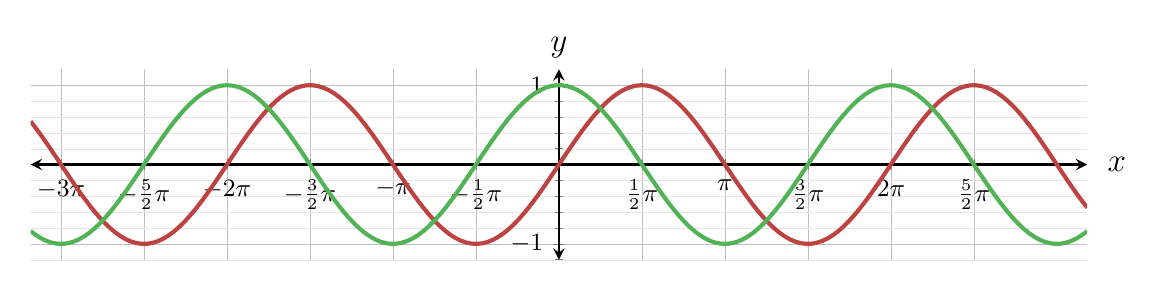
\begin{tikzpicture}
		\begin{axis}[
				graph2d,
				width=15cm, height=4cm,
				xmin=-10, xmax=10,
				ymin=-1.2, ymax=1.2,
				xtick={-9.425,-7.854,...,9.425,10.996},
				xticklabels={$-3\pi$, $-\frac{5}{2}\pi$, $-2\pi$, $-\frac{3}{2}\pi$, $-\pi$, $-\frac{1}{2}\pi$, , $\frac{1}{2}\pi$, $\pi$, $\frac{3}{2}\pi$, $2\pi$, $\frac{5}{2}\pi$, $3\pi$},
				domain=-10:10,
			]
			\addplot[function, xred] {sin(deg(\x))};
			\addplot[function, xgreen] {cos(deg(\x))};
		\end{axis}
	\end{tikzpicture}
	\caption{The graphs of \textcolor{xdarkred}{$\sin(x)$} and \textcolor{xdarkgreen}{$\cos(x)$} for $x\in[-10,10]$. Note how the graph of \textcolor{xdarkgreen}{$\cos(x)$} is ``lagging'' behind the graph of \textcolor{xdarkred}{$\sin(x)$} by $\pi/2$.}
	\label{fig:tan graph}
\end{figure}

\begin{figure}
	\centering
	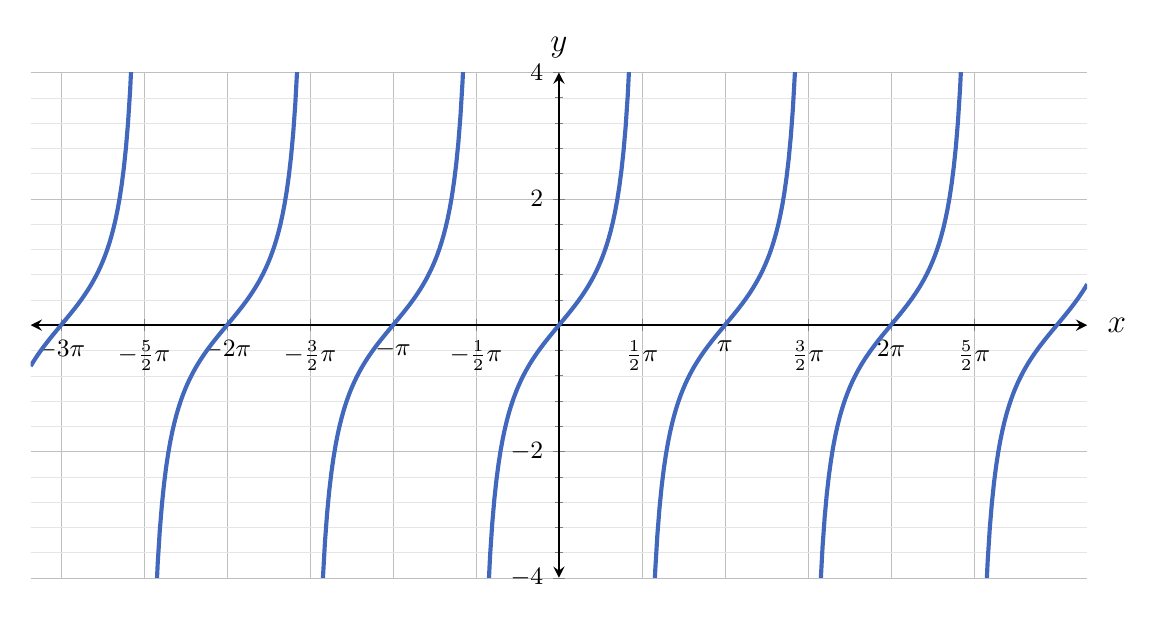
\begin{tikzpicture}
		\begin{axis}[
				graph2d,
				width=15cm, height=8cm,
				xmin=-10, xmax=10,
				ymin=-4, ymax=4,
				xtick={-9.425,-7.854,...,9.425,10.996},
				xticklabels={$-3\pi$, $-\frac{5}{2}\pi$, $-2\pi$, $-\frac{3}{2}\pi$, $-\pi$, $-\frac{1}{2}\pi$, , $\frac{1}{2}\pi$, $\pi$, $\frac{3}{2}\pi$, $2\pi$, $\frac{5}{2}\pi$, $3\pi$},
				domain=-10:10,
				restrict y to domain=-5:5,
				samples=500,
			]
			\addplot[function, xblue] {tan(deg(\x))};
		\end{axis}
	\end{tikzpicture}
	\caption{The graphs of $\tan(x)$ on the domain $[-3\pi,3\pi]$.}
	\label{fig:sin and cos graphs}
\end{figure}

\subsection{Identities}
The following are some useful facts and connections between trigonometric functions:
\begin{itemize}
	\item Pythagorean identity:
		\begin{equation}
			\sin^{2}(\theta) + \cos^{2}(\theta) = 1
		\end{equation}
	
	\item Symmetry/Antisymmetry:
		\begin{align}
			\sin(-\theta) &= -\sin(\theta).\\
			\cos(-\theta) &= \cos(\theta).\\
			\tan(-\theta) &= -\tan(\theta).
		\end{align}
	
	\item Tangent from sine and cosine:
		\begin{equation}
			\tan(\theta)=\frac{\sin(\theta)}{\cos(\theta)}.
		\end{equation}
	
	\item Phase between sine and cosine:
		\begin{align}
			\sin\left(\theta\pm\frac{\pi}{2}\right) &= \pm\cos(\theta).\\
			\cos\left(\theta\pm\frac{\pi}{2}\right) &= \mp\sin(\theta).
		\end{align}
	
	\item Half-period shift:
		\begin{align}
			\sin(\theta+\pi) &= -\sin(\theta).\\
			\cos(\theta+\pi) &= -\cos(\theta).
		\end{align}
	
	\item Angle sum:
		\begin{align}
			\sin(\alpha\pm\beta) &= \sin(\alpha)\cos(\beta)\pm\cos(\alpha)\sin(\beta).\\
			\cos(\alpha\pm\beta) &= \cos(\alpha)\cos(\beta)\mp\sin(\alpha)\sin(\beta).
		\end{align}
	
	\item Double angle:
		\begin{align}
			\sin(2\theta) &= 2\sin(\theta)\cos(\theta) = \frac{2\tan \left( \theta \right)}{1+\tan^{2} \left( \theta \right)}.\\
			\cos(2\theta) &= 1-2\sin^{2}(\theta) = \frac{1-\tan^{2} \left( \theta \right) }{1+\tan^{2} \left( \theta \right)}.
			\label{eq:double_angles}
		\end{align}
	
	\item Half angle:
		\begin{align}
			\sin\left( \frac{\theta}{2} \right) &= \pm\sqrt{\frac{1-\cos(\theta)}{2}}.\\
			\cos\left( \frac{\theta}{2} \right) &= \pm\sqrt{\frac{1+\cos(\theta)}{2}}.\\
			\tan\left( \frac{\theta}{2} \right) &= \frac{\sin(\theta)}{1+\cos(\theta)}.
		\end{align}
	
	\item Product to sum:
		\begin{align}
			\sin(\theta)\sin(\varphi) &= \frac{1}{2}\left[ \cos(\theta-\varphi)-\cos(\theta+\varphi) \right].\\
			\cos(\theta)\cos(\varphi) &= \frac{1}{2}\left[ \cos(\theta-\varphi)+\cos(\theta+\varphi) \right].\\
			\sin(\theta)\cos(\varphi) &= \frac{1}{2}\left[ \sin(\theta+\varphi) + \sin(\theta-\varphi) \right].\\
			\tan(\theta)\tan(\varphi) &= \frac{\cos(\theta-\varphi)-\cos(\theta+\varphi)}{\cos(\theta-\varphi)+\cos(\theta+\varphi)}.
			\label{eq:trig product to sum}
		\end{align}

	\item Sum to product:
		\begin{align}
			\sin(\theta)\pm\sin(\varphi) &= 2\sin\left( \frac{\theta\pm\varphi}{2} \right)\cos\left( \frac{\theta\mp\varphi}{2} \right).\\
			\cos(\theta)+\cos(\varphi) &= 2\cos\left( \frac{\theta+\varphi}{2} \right)\cos\left( \frac{\theta-\varphi}{2} \right).\\
			\cos(\theta)-\cos(\varphi) &= -2\cos\left( \frac{\theta+\varphi}{2} \right)\cos\left( \frac{\theta-\varphi}{2} \right).\\
			\tan(\theta)\pm\tan(\varphi) &= \frac{\sin(\theta\pm\varphi)}{\cos(\theta)\cos(\varphi)}.
			\label{eq:trig sum to product}
		\end{align}
\end{itemize}

\subsection{Useful theorems}
The area $S$ of a triangle $\triangle ABC$ can be calculated using the length $L$ any side of the triangle (in this context called a \emph{base}) and the height $h$ to its opposing vertex (see \autoref{fig:area of a triangle}):
\begin{equation}
	S = \frac{1}{2}Lh.
	\label{eq:area of a triangle}
\end{equation}

\begin{figure}
	\centering
	\begin{tikzpicture}
		\coordinate (A) at (-2,1);
		\coordinate (B) at (1,3.5);
		\coordinate (C) at (2,1);
		\coordinate (D) at (B|-C);
		\draw[very thick, fill=xblue!20] (A) node[left] {$A$} -- (B) node[above] {$B$} node[midway, above left] {$c$} -- node[midway, right] {$a$} (C) node[right] {$C$} -- cycle node[midway, below] {$b$};
		\draw[thick, dashed] (B) -- (D) node[midway, left] {$h$};
		\draw[thick] (D) -- ++(0.2,0) -- ++(0,0.2) -- ++(-0.2,0);
		\pic[draw, thick, angle radius=11mm, angle eccentricity=0.7, "$\alpha$"] {angle=C--A--B};
	\end{tikzpicture}
	\caption{The area of a triangle using the side $b$ as a base, and its corresponding height to the point $B$. The angle opposing the side $A$ is marked as $\alpha$.}
	\label{fig:area of a triangle}
\end{figure}

The triangle with sides $cbh$ is a right triangle, $c$ being its hypotenuse. We can therefore infer the size of $h$ using $\alpha$:
\begin{equation}
	h = c\sin(\alpha).
	\label{eq:first equation in law of sines}
\end{equation}
Substituting this back to \autoref{eq:area of a triangle} yields that the area of the triangle is
\begin{equation}
	S = \frac{1}{2}bc\sin(\alpha).
	\label{eq:area using sin theta}
\end{equation}
There is nothing special about choosing the side $b$ as a base: we can also use $a$ or $c$ for the calculation. This will yield, respectively,
\begin{align}
	S &= \frac{1}{2}ac\sin(\gamma),\\
	S &= \frac{1}{2}ac\sin(\beta),
	\label{eq:}
\end{align}
where $\beta$ is the angle opposing $b$ and $\gamma$ is the angle opposing $c$. Since $S$ is the same in all cases, we simply multiply each of the area equations by $2$ and divide by $abc$, which yields
\begin{equation}
	\frac{\sin(\alpha)}{a} = \frac{\sin(\beta)}{b} = \frac{\sin(\gamma)}{c},
	\label{eq:law of sines}
\end{equation}
i.e. in a triangle, the ratio between any side and the sine of its opposing angle is always the same no matter which side we choose. This theorem is called the \emph{law of sines}.

\begin{example}{Law of sines}{}
	Given the triangle $\triangle ABC$ below, what are $\beta$ and $b$?

	\vspace{2em}
	\centering
	\begin{tikzpicture}
		\coordinate (A) at (2,-1);
		\coordinate (B) at (2,3);
		\coordinate (C) at (-1,4);
		% a=3.15, b=5.83, c=4
		% α=30.79 β=108.67 γ=40.54
		\draw[very thick, fill=xpurple!40] (A) -- (B) node[midway, right] {$c$} -- node[midway, above right] {$a=3.15$} (C) -- cycle node[midway, below left] {$b$};

		% "local bounding box" gives the pic its label
		\pic[local bounding box=alpha, draw, thick, angle radius=11mm, angle eccentricity=0.7, "$\alpha$"] {angle=B--A--C};
		\pic[local bounding box=beta, draw, thick, angle radius=7mm, angle eccentricity=0.6, "$\beta$"] {angle=C--B--A};
		\pic[local bounding box=gamma, draw, thick, angle radius=11mm, angle eccentricity=0.7, "$\gamma$"] {angle=A--C--B};

		\node[above right of=alpha, xshift=2mm] (alphatxt) {$\ang{30.79}$};
		\node[below left of=gamma, xshift=-2mm] (gammatxt) {$\ang{40.54}$};
		\draw[vector, thick] (alphatxt.south) to [out=-90, in=0] (alpha);
		\draw[vector, thick] (gammatxt.north) to [out=90, in=180] (gamma);
	\end{tikzpicture}

	\vspace{1em}
	\flushleft
	Since all angles in a triangle must add up to $\ang{180}$,
	\[
		\beta=\ang{180}-\ang{30.79}-\ang{40.54}=\ang{108.67}.
	\]

	Using the law of sines,
	\[
		b = \frac{a}{\sin(\alpha)}\cdot\sin(\beta) = \frac{3.15}{\sin(\ang{30.79})}\cdot\sin(\ang{108.67}) \approx 5.83,
	\]
	and
	\[
		c = \frac{a}{\sin(\alpha)}\cdot\sin(\gamma) = \frac{3.15}{\sin(\ang{30.79})}\cdot\sin(\ang{40.54}) \approx 4.
	\]
\end{example}

\begin{note}{Ambiguity of solutions}{}
	The above example reveals an issue that might arise due to the symmetrical nature of $\sin(x)$ around $x=\pi$ ($\ang{180}$): say we wanted to calculate $\beta$ using the law of sines instead of by using $\beta=\ang{180}-\alpha-\gamma$. In this case we would solve the equation
	\[
		\frac{\sin(\alpha)}{a} = \frac{\sin(\beta)}{b},
	\]
	which would result in $\beta=\arcsin\left( \frac{b\sin(\alpha)}{a}  \right)=\arcsin\left( 0.95 \right)$. However, two angles can fit this requirement: the sines of $\ang{71.34}$ and $\ang{108.67}$ are both equal to $0.95$! Therefore, we must be careful when using the law of sine and make sure we always choose values that make sense (e.g. such that all angles add up to $\ang{180}$).
\end{note}

Of course, the sine function is not unique in having its own named ``Law'': another useful theorem is the so-called \emph{law of cosines} (also \emph{al-Kashi's theorem}). This theorem states that given a triangle with sides $a,b,c$ and an angle $\gamma$ opposing $c$,
\begin{equation}
	c^{2} = a^{2} + b^{2} - 2ab\cos(\gamma).
	\label{eq:law of cosines}
\end{equation}

Much like the law of sines, the choice of angle does not matter, as long as we plug the correct sides to the equation: for $\alpha$ and $\beta$ being the angles opposing to $a$ and $b$ respectively,
\begin{align}
	a^{2} &= b^{2} + c^{2} - 2bc\cos(\alpha),\nonumber\\
	b^{2} &= a^{2} + c^{2} - 2ac\cos(\beta).
\end{align}

If the triangle in question is a right triangle then one of the angles is equal to $\ang{90}$. Without loss of generality, let us assume that this is $\gamma$. Since $\cos(\ang{90})=0$ we get that in the case of a right triangle
\begin{equation}
	c^{2} = a^{2} + b^{2},
	\label{eq:pythagorean theorem from law of cosines}
\end{equation}
i.e. we retrieve back the Pythagorean theorem.

\begin{example}{Law of cosines}{}
	Calculate all angles in the following triangle:

	\vspace{2em}
	\centering
	\begin{tikzpicture}
		\coordinate (A) at (-3,0);
		\coordinate (B) at (2,-1);
		\coordinate (C) at (-1,3);
		% a=5 b=3.61 c=5.1
		% α=70.55 β=67.58 γ=41.87
		\draw[very thick, fill=xgreen!50] (A) -- (B) node[midway, below left] {$c=5.1$} -- node[midway, above right] {$a=5$} (C) -- cycle node[midway, above left] {$b=3.61$};

		% "local bounding box" gives the pic its label
		\pic[local bounding box=alpha, draw, thick, angle radius=9mm, angle eccentricity=0.6, "$\alpha$"] {angle=B--A--C};
		\pic[local bounding box=beta, draw, thick, angle radius=11mm, angle eccentricity=0.7, "$\beta$"] {angle=C--B--A};
		\pic[local bounding box=gamma, draw, thick, angle radius=9mm, angle eccentricity=0.6, "$\gamma$"] {angle=A--C--B};
	\end{tikzpicture}

	\vspace{1em}
	\flushleft
	Using the law of cosines:
	\begin{align*}
		\cos(\gamma) &= \frac{c^{2}-b^{2}-a^{2}}{-2ab} = \frac{5.1^{2}-3.61^{2}-5^{2}}{-2\cdot5\cdot3.61} \approx 0.33302\Rightarrow \gamma=\ang{70.54},\\
		\cos(\beta) &= \frac{b^{2}-a^{2}-c^{2}}{-2ac} = \frac{3.61^{2}-5^{2}-5.1^{2}}{-2\cdot5\cdot5.1} \approx 0.74466\Rightarrow \beta=\ang{41.87},\\
		\cos(\alpha) &= \frac{a^{2}-b^{2}-c^{2}}{-2cb} = \frac{5^{2}-3.61^{2}-5.1^{2}}{-2\cdot5.1\cdot3.61} \approx 0.38135\Rightarrow \alpha=\ang{67.58}.
	\end{align*}
\end{example}

\tbw{
  Consider showing this nice geometric reasoning behind sin(2x)=2sin(x)cos(x):
  https://www.youtube.com/watch?v=mKPgmaoGC4o
}

%\begin{figure}
%	\centering
%	\begin{tikzpicture}
%		\pgfmathsetmacro{\ax}{4.5}
%		\pgfmathsetmacro{\un}{3.5}
%		\pgfmathsetmacro{\th}{35}
%		\coordinate (D) at ({\un*cos(\th)},0);
%
%		\filldraw[xred!35] (A) -- (\un,0) arc (0:90:\un);
%		\filldraw[xblue!35] (A) -- (0,\un) arc (90:180:\un);
%		\filldraw[xgreen!35] (A) -- (-\un,0) arc (180:270:\un);
%		\filldraw[xorange!35] (A) -- (0,-\un) arc (270:360:\un);
%		\node at ({ \un/2.5},{ \un/2.5}) {\Huge$1$};
%		\node at ({-\un/2.5},{ \un/2.5}) {\Huge$2$};
%		\node at ({-\un/2.5},{-\un/2.5}) {\Huge$3$};
%		\node at ({ \un/2.5},{-\un/2.5}) {\Huge$4$};
%		
%		\draw[thick] (A) circle (\un);
%		\draw[vector, <->] (-\ax,0) -- (\ax,0) node [right] {\Large$x$};
%		\draw[vector, <->] (0,-\ax) -- (0,\ax) node [above] {\Large$y$};
%		\filldraw (A) circle (2pt) node[below right] {$(0,0)$};
%		\filldraw (\un,0) circle (2pt) node[below right] {$(1,0)$};
%		\filldraw (0,\un) circle (2pt) node[above right] {$(0,1)$};
%		\filldraw (-\un,0) circle (2pt) node[below left] {$(-1,0)$};
%		\filldraw (0,-\un) circle (2pt) node[below right] {$(0,-1)$};
%	\end{tikzpicture}
%	\caption{The different quadrants of the unit circle.}
%	\label{fig:unit_circle_quadrants}
%\end{figure}

%\begin{table}
%	\caption{Text}
%	\label{tab:quadrants_trig_vals}
%	\centering
%	\begin{tabular}{lll}
%		\toprule
%		Quadrant & $\cos(\theta)=x$ & $\sin(\theta)=y$\\
%		\midrule
%		\rowcolor{xred!35}1 & $\left[ 0,1 \right]$ & $\left[ 0,1 \right]$\\
%		\rowcolor{xblue!35}2 & $\left[-1,0 \right]$ & $\left[ 0,1 \right]$\\
%		\rowcolor{xgreen!35}3 & $\left[-1,0 \right]$ & $\left[-1,0 \right]$\\
%		\rowcolor{xorange!35}4 & $\left[ 0,1 \right]$ & $\left[-1,0 \right]$\\
%		\bottomrule
%	\end{tabular}
%\end{table}


\pgfkeys{
	/pgfplots/complex plane/.style={
	axis x line=middle,
	axis y line=middle,
	xlabel=$\Re$,
	ylabel=$\Im$,
	every axis x label/.style={
		at={(ticklabel* cs:1.02)},
		anchor=west,
	},
	every axis y label/.style={
		at={(ticklabel* cs:1.02)},
		anchor=south,
	},
	axis line style={stealth-stealth, thick},
	label style={font=\large},
	tick label style={font=\large},
	samples=100,
	xmin=-3, xmax=3,
	ymin=-3, ymax=3,
	domain=-3:3,
	grid=both,
	major grid style={black!5},
}}

\section{Complex Numbers}
\subsection{Algebraic approach}
Real numbers, while being extremely useful, are not complete - they can't solve all equations involving numbers. For example, the equation
\begin{equation}
	x^{2} + 1 = 0
	\label{eq:no_real_solutions}
\end{equation}
has no real solutions, since there can be no real number $x$ such that $x^{2}=-1$. However, we can choose to define a new number, $i=\sqrt{-1}$ and using it to build a new number system. This system is of course the set of complex numbers, $\mathbb{C}$. It is defined as the set of all $z$ such that
\begin{equation}
	z = a+ib,
	\label{eq:complex_number}
\end{equation}
where $a,b\in\mathbb{R}$ and $i=\sqrt{-1}$. We call $a$ the \emph{real component} of $z$, and $b$ its \emph{imaginary component}\footnote{There is nothing more ``real'' about real numbers than imaginary numbers, but unfortunately that's the terminology we're stuck with \shrug}. These numbers appear a lot all throughout the exact sciences (but especially in physics and engineering), so we must at the very least learn their basic properties.

It is not so obvious that we can add two different kinds of numbers together, but it works (the linear algebra chapter sheds more light on this idea). What is important is that we always keep these two parts separated. We see this when we add together two complex numbers $z_{1},z_{2}$:
\begin{equation}
	z = z_{1}+z_{2} = \left( a_{1}+b_{1}i \right) + \left( a_{2}+b_{2}i \right) = \left( a_{1}+a_{2} \right) + \left( b_{1}+b_{2} \right)i.
	\label{eq:complex_addition}
\end{equation}
The real part of $z$ is therefore $a_{1}+b_{1}$, and its imaginary part is $b_{1}+b_{2}$.

What happens when we multiply two complex numbers? Let's check:
\begin{align}
	z = z_{1}z_{2} &= \left( a_{1}+b_{1}i \right)\left( a_{2}+b_{2}i \right)\nonumber\\
	&= a_{1}a_{2} + a_{1}b_{2}i + a_{2}b_{1}i + b_{1}b_{2}i^{2}\nonumber\\
	&= a_{1}a_{2} + a_{1}b_{2}i + a_{2}b_{1}i - b_{1}b_{2}\nonumber\\
	&= \left( a_{1}a_{2} - b_{1}b_{2} \right) + \left( a_{1}b_{2} + a_{2}b_{1} \right)i.
	\label{eq:complex_product}
\end{align}
We see that we can still separate the real part and imaginary part of the result. What happens in the case of two real numbers? For real numbers $b=0$, and thus \eqref{complex_product} devolves to $z=a_{1}a_{2}\in\mathbb{R}$, which is exactly what we expect: multiplying two real numbers yields their product, which is a real number. Notice that this doesn't happen with purely imaginary numbers: multiplying together two imaginary numbers (i.e. numbers for which $a=0$) results in a real number. Will get to understand why this happens very soon.

When discussing real numbers sometimes we like to refer to their \textit{magniture}, i.e. their absolute value. With complex numbers this is defined as
\begin{equation}
	|z| = \sqrt{a^{2}+b^{2}},
	\label{eq:complex_magnitude}
\end{equation}
i.e. in a sense, to get the magnitude of a complex number we imagine its two components as being perpendicular and calculate the length of the resulting hypotenous (cf.\ the Pythagorean theorem). In fact, this is one very useful interpertation of complex numbers, which we will explore in depth in the next subsection.

A very important operation that can be applied to complex numbers is \emph{conjugation}. The conjugate of a complex number $z=a+bi$ is defined as
\begin{equation}
	\conj{z} = a-bi,
	\label{eq:complex_conjugation}
\end{equation}
i.e. conjugating a number is simply negating its imaginary part. When we multiply a complex number by its own complex conjugate we get
\begin{equation}
	z\conj{z} = (a+bi)(a-bi) = a^{2} + abi - abi - b^{2}i^{2} = a^{2}+b^{2},
	\label{eq:conjugate_product}
\end{equation}
i.e. $z\conj{z} = |z|^{2}$. The inverse of a complex number can be expressed as
\begin{equation}
	z^{-1} = \frac{\conj{z}}{|z|^{2}}.
	\label{eq:complex_inverse}
\end{equation}

\subsection{Geometric approach}
As alluded to in the previous subsection, we can interpret a complex number $z=a+bi$ as two components in a 2-dimentional space, in which the horizontal axis represents real components, and the vertical access represents imaginary components:
\begin{figure}[H]
	\centering
	\begin{tikzpicture}
		\tikzstyle{every node}=[font=\large]
		\pgfmathsetmacro{\a}{2}
		\pgfmathsetmacro{\b}{2.5}
		\pgfmathsetmacro{\t}{atan2(\b,\a)}
		\begin{axis}[
			complex plane,
			width=10cm, height=10cm,
			xtick={-3,-2.5,...,3},
			xticklabels={},
			extra x ticks={\a},
			extra x tick labels={$a$},
			ytick={-3,-2.5,...,3},
			yticklabels={},
			extra y ticks={\b},
			extra y tick labels={$b$},
		]
		\draw[very thick, dashed, xred] (0,0) -- node[midway, above, rotate=\t] {$|z|=\sqrt{a^{2}+b^{2}}$} (\a,\b);
		\addplot+[black, only marks, mark=*, mark options={scale=0.5, fill=black}, text mark as node=true] coordinates {
			(\a,\b)
		} node[above] {$z=a+bi$};
		\end{axis}
	\end{tikzpicture}
\end{figure}

Drawing a line from $z$ to $a$ (on the real axis) creates a right triangle. We can then define $\theta$ to be the angle near the origin and $r$ the length of the hypotenous:
\begin{figure}[H]
	\centering
	\begin{tikzpicture}
		\tikzstyle{every node}=[font=\large]
		\pgfmathsetmacro{\a}{2}
		\pgfmathsetmacro{\b}{2.5}
		\pgfmathsetmacro{\t}{atan2(\b,\a)}
		\begin{axis}[
			complex plane,
			width=10cm, height=10cm,
			xtick={-3,-2.5,...,3},
			xticklabels={},
			extra x ticks={\a},
			extra x tick labels={$a$},
			ytick={-3,-2.5,...,3},
			yticklabels={},
			extra y ticks={\b},
			extra y tick labels={$b$},
		]
		\draw[very thick, xred] (0,0) -- node[midway, above, rotate=\t] {$r$} (\a,\b);
		\addplot+[black, only marks, mark=*, mark options={scale=0.5, fill=black}, text mark as node=true] coordinates {
			(\a,\b)
		} node[right] {$z$};
		\draw[thick, dashed] (\a,\b) -- (\a,0);
		\draw[thick] ({\a-0.25},0) -- ({\a-0.25},0.25) -- (\a,0.25);
		\draw[very thick, xpurple] (0.75,0) arc (0:\t:0.75);
		\node[xpurple] at ({cos(\t/2)},{sin(\t/2)}) {$\theta$};
		\end{axis}
	\end{tikzpicture}
\end{figure}

Using \eqref{xy_P} the real and imaginary components of $z$ are
\begin{align}
	a &= r\cos(\theta),\nonumber\\
	b &= r\sin(\theta),
	\label{eq:complex_components}
\end{align}
and $z$ can be re-written as
\begin{equation}
	z = r\left( \cos(\theta) + i\sin(\theta) \right).
	\label{eq:complex_geometric_form}
\end{equation}


\end{document}
